\documentclass[journal=jacsat,manuscript=article]{achemso}
\usepackage[T1]{fontenc} % Use modern font encodings
\usepackage{amsmath} 
\usepackage{bookmark}
\usepackage{booktabs}
\usepackage{xspace}
\usepackage{relsize}
\usepackage{tabularx}
\usepackage{multirow}
\usepackage{multicol}
\usepackage{xcolor}

\usepackage{hyperref}
\hypersetup{
    colorlinks=true,        
    linkcolor=blue,        
    citecolor=blue,       
    urlcolor=blue           
}
\usepackage[capitalise]{cleveref} % load after hyperref package
\captionsetup[figure]{labelfont=bf}
\captionsetup[table]{labelfont=bf}


\tolerance=1
\usepackage[none]{hyphenat}
\emergencystretch=\maxdimen
%%%%%%%%%%%%%%%%%%%%%%%%%%%%%%%%%%%%%%%%%%%%%%%%%%%%%%%%%%%%%%%%%%%%%
\newcommand*\mycommand[1]{\texttt{\emph{#1}}}
%%%%%%%%%%%%%%%%%%%%%%%%%%%%%%%%%%%%%%%%%%%%%%%%%%%%%%%%%%%%%%%%%%%%%
\author{Ubeiden Cifuentes Samboni}
\author{Agustina Godino}
\author{José L. Barra}
\author{Rafael G. Oliveira}
\author{Guillermo G. Montich}
\email{guillermo.montich@unc.edu.ar}
\affiliation{Centro de Investigaciones en Química Biológica de Córdoba (CIQUIBIC), CONICET, Departamento de Química Biológica Ranwel Caputto, Facultad de Ciencias Químicas, Universidad Nacional de Córdoba, Ciudad Universitaria, Córdoba X5000HUA, Argentina}
%%%%%%%%%%%%%%%%%%%%%%%%%%%%%%%%%%%%%%%%%%%%%%%%%%%%%%%%%%%%%%%%%%%%%


\title{Interactions of Integrin $\alpha$IIb$\beta$3 Transmembrane-Cytoplasmic Segments with Lipids in Langmuir Monolayers. Surface, Mechanical and Morphological Properties}

%%%%%%%%%%%%%%%%%%%%%%%%%%%%%%%%%%%%%%%%%%%%%%%%%%%%%%%%%%%%%%%%%%%%%
% \keywords{Integrin, Transmembrane Protein, Lipids, Surface Potential, Langmuir Monolayers, Compressibility, Brewster Angle Microscopy}
%%%%%%%%%%%%%%%%%%%%%%%%%%%%%%%%%%%%%%%%%%%%%%%%%%%%%%%%%%%%%%%%%%%%%
\begin{document}

\begin{tocentry}
    \centering
    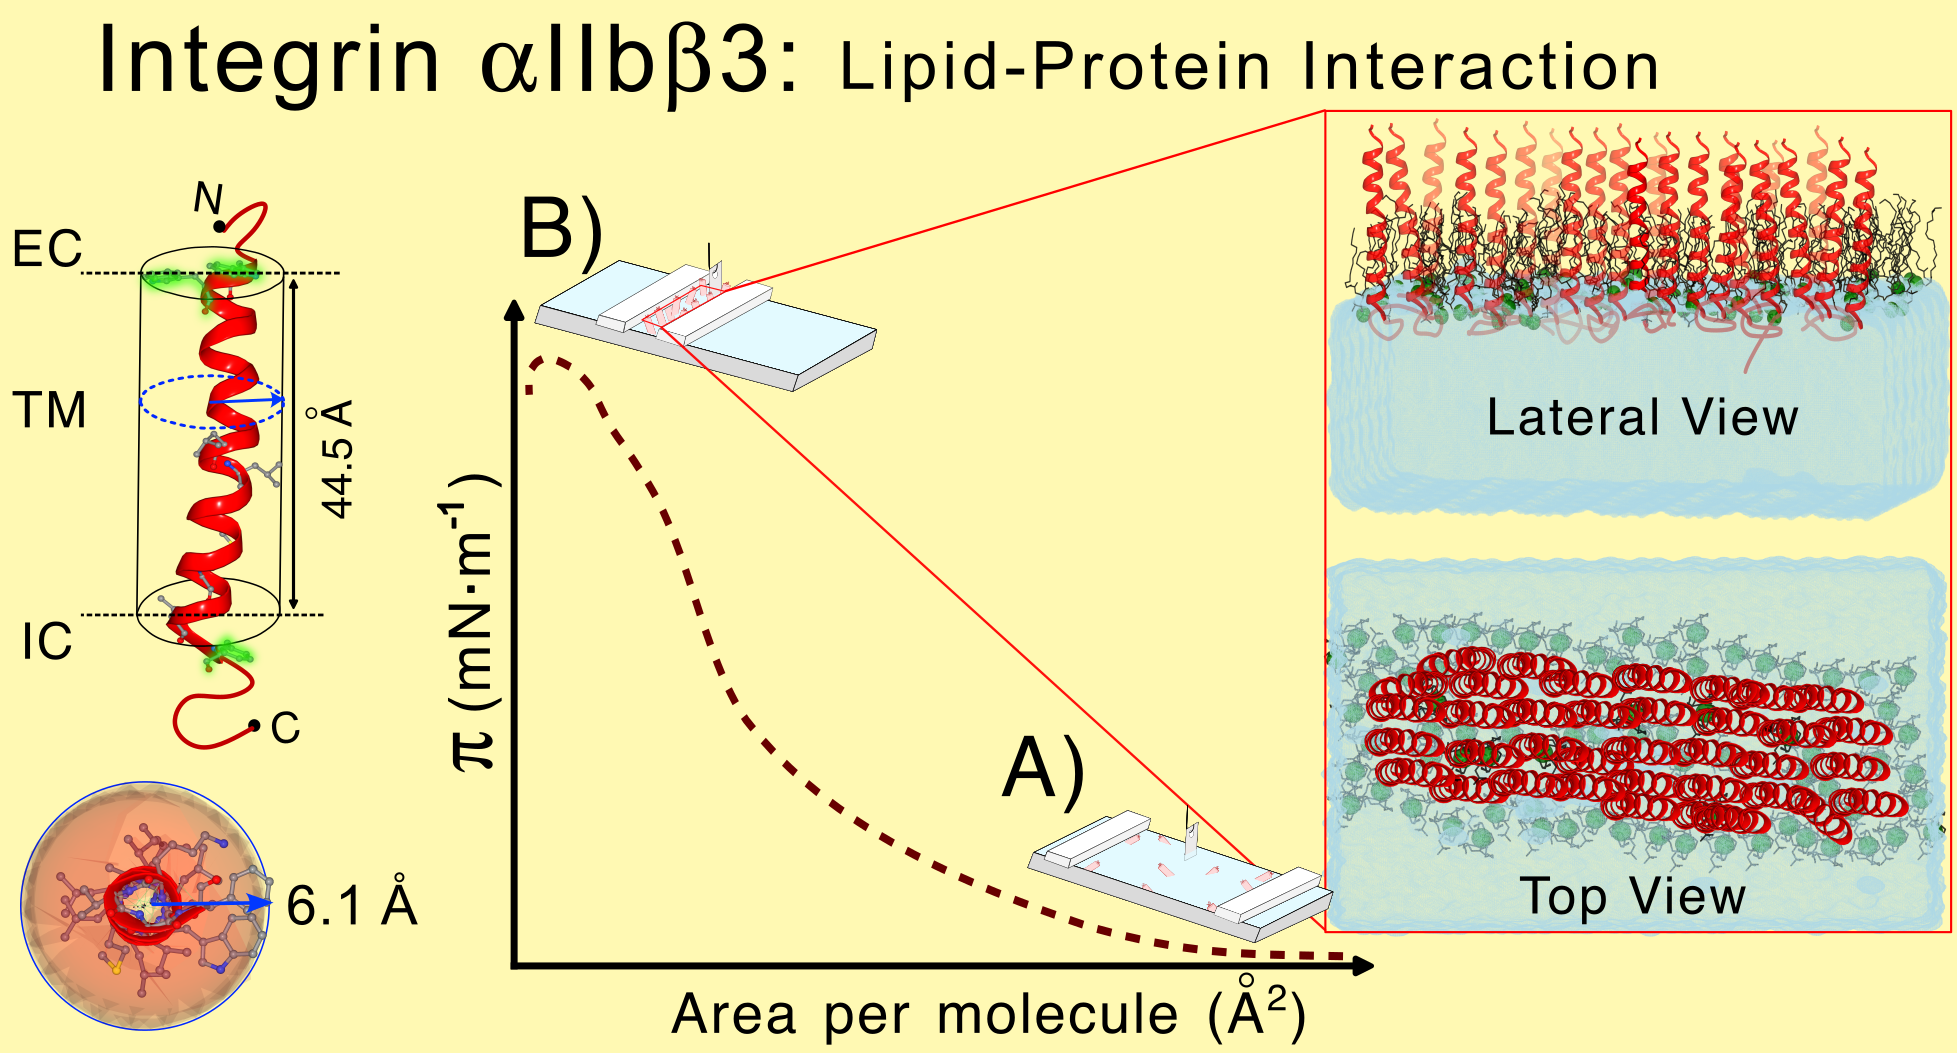
\includegraphics[width=1\linewidth, keepaspectratio]{tocFig.png}
\end{tocentry}

%%%%%%%%%%%%%%%%%%%%%%%%%%%%%%%%%%%%%%%%%%%%%%%%%%%%%%%%%%%%%%%%%%%%%


\begin{abstract}
Integrins are transmembrane receptors that mediate cell adhesion and signaling. They perform allosteric rearrangements to transmit external signals to intracellular regions, while intracellular signaling events can also influence their extracellular behavior. 
The $\alpha$IIb$\beta$3 integrin, found in human platelets, is involved in thrombosis and hemostatic processes. Protein–lipid interactions can regulate membrane organization, influencing integrin conformational states and downstream signaling.
In this study, we expressed and purified peptides comprising the transmembrane (TM), the intracellular (IC) segments and a small portion of the extracellular segments (EC) of $\alpha$IIb and $\beta$3 integrin and studied the surface behaviour of the pure peptides and their mixtures with 1–palmitoyl–2–oleoyl–\textit{sn}–glycero–3–phosphocholine (POPC), with a mixture of the zwitterionic lipid POPC with the anionic 1–palmitoyl–2–oleoyl–\textit{sn}–glycero–3–phosphoglycerol (POPG), and with 1,2–dipalmitoyl–\textit{sn}–3–glycerophosphocholine (DPPC) using Langmuir monolayers and Brewster angle microscopy (BAM). The peptides formed stable monolayers at the air/water interface. Mixtures with the unsaturated lipid POPC and a mixture of POPC–POPG showed negative deviation of ideal mixing, while the mixtures with the saturated DPPC deviated positively from ideal mixing. BAM imaging revealed that pure peptides formed a continuous network of reflective threads surrounding dark patches. In the mixtures with DPPC the threads were fragmented while POPC mixtures maintained the connectivity. These findings showed that these peptides from integrin $\alpha$IIb$\beta$3 have different interactions with different lipids, which could have implications for integrin activation and function in platelet membranes.

\end{abstract}


\subsubsection{Keywords}
Integrin, Transmembrane Protein, Lipids, Surface Potential, Langmuir Monolayers, Compressibility, Brewster Angle Microscopy
%%%%%%%%%%%%%%%%%%%%%%%%%%%%%%%%%%%%%%%%%%%%%%%%%%%%%%%%%%%%%%%%%%%%%
%% Start the main part of the manuscript here.
%%%%%%%%%%%%%%%%%%%%%%%%%%%%%%%%%%%%%%%%%%%%%%%%%%%%%%%%%%%%%%%%%%%%%
\section{Introduction}
    Integrin are membrane proteins that mediate the interactions and attachments between cells and between cells and the extracellular matrix. They are key proteins in the organization of tissues and in the transduction of information between the cell and its environment in multicellular organisms. They are heterodimers constituted by an $\alpha$ and a $\beta$ subunit, these monomers are type I proteins with a large extracellular segment (EC), a single helical transmembrane (TM) segment and a small intracellular (IC) segment \cite{Tamkun1986,2010_Barczyk}. Integrins can transduce information through the plasma membrane outside–in and inside–out the cell \cite{Iwamoto2015, Campbell2011}. They have available several conformation states and can switch between them in processes coupled to ligands binding, both in the extracellular or intracellular environment. \cite{Luo2003,Li2017,Litvinov2004,Springer2012}.

    Integrin $\alpha$IIb$\beta$3, found in the plasma membrane of human platelets, megakaryocytes, mastocytes, and basophil cells, plays an active role in platelet aggregation and clot formation \cite{Chen1997,Pabla1999,Kaneva2019}. The structure of the whole protein was described by Adair and Yeager \cite{Adair2002} and by Vinogradova et al. \cite{Vinogradova2002} using cryomicroscopy. NMR studies performed in lipid bicelles have described the structure and relative orientation of the TM segments \cite{Lau2009,Yang2009,Ulmer2010}. The binding of ligands, like talin, to the IC segment of the dimer shifts the conformation to an active state: the TM segments are dissociated and the EC segment acquires a conformation suitable for binding to fibrinogen \cite{Ugarova2001,Mosesson2005}. In the inactive state, TM segments are closely bound through ridge–valley interactions \cite{Zhu2009} in the classical way early described by Chothia et al. \cite{1977_Chothia} through the sequences KVGFFKR in $\alpha$IIb and KLLITIHD in $\beta$3.

	Lipids are active components in the regulation of membrane protein activities. The behaviour and functions of membrane proteins is controlled not only by the interactions with specific lipids but also by the global properties of the membrane such as compressibility, fluidity, electrostatic interactions, membrane curvature and the proper matching between hydrophobic domains \cite{1997_Cantor,2004_Morten} even for non–integral membrane proteins \cite{2021_Oliveira}. 
    Considering that the activation of $\alpha$IIb$\beta$3 requires the movement of $\alpha$–helix segments within the lipid environment of the plasma membrane, we are interested in characterizing the interactions of these segments with lipids. In this work we studied the interactions of two peptides comprising the IC, the TM and a small portion of the EC segments of $\alpha$IIb and $\beta$3 monomers of integrin $\alpha$IIb$\beta$3 with lipids in monolayers at the air/water interface. 
    By measuring compressibility, surface potential, deviations from the ideal mixing behaviour, which are global, macroscopic properties of the monolayer, we can obtain information about the mutual influence between peptides and lipids. BAM was used to study the microscopic organization of the monolayers. We studied the monolayers of pure peptides, pure lipids and lipid–peptides mixtures. Among the many properties of the lipid monolayers that can have an influence on the interactions with the peptides, we focused on the phase state of the lipid and the electrostatic charge. For these reasons we studied the interactions with a zwitterionic lipid in the liquid expanded (LE) state, 1–palmitoyl–2–oleoyl–\textit{sn}–glycero–3–phosphocholine (POPC), a mixture of the zwitterionic lipid POPC with the anionic 1–palmitoyl–2–oleoyl–\textit{sn}–glycero–3–phosphoglycerol (POPG), both in the liquid expanded state (PC–PG mixture), and a zwitterionic lipid that undergoes a phase transition between the LE and the liquid condensed (LC) phase, 1,2–dipalmitoyl–\textit{sn}–3–glycerophosphocholine (DPPC). 
 
    The Langmuir monolayer is a powerful experimental approach for investigating molecular areas, dipolar organization, and phase states under controlled conditions such as surface pressure and surface area. Although lipid monolayers differ in geometry and structure from bilayers they are valuable for studying the fundamentals of lipid–protein interactions. In this study, we show that monolayers composed of pure $\alpha$IIb and $\beta$3 peptides form domain networks that are differentially influenced by specific lipids, indicating different interaction profiles. While these findings cannot be directly extrapolated to the behaviour of TM peptides in complex, asymmetric plasma membranes, they provide an insight into how lipids interact with TM peptides.


%%%%%%%%%%%%%%%%%%%%%%%%%%%%%%%%%%%%%%%%%%%%%%%%%%%%%%%%%%%%%%%%%%%%%
\section{Experimental Section}\label{sec:expeSection}

\textit{Chemicals and Reagents}. POPC, POPG and DPPC were purchased from Avanti Polar Lipids (Alabaster, AL, USA). The lipids were used without further purification. Chloroform and methanol, high–performance liquid chromatography (HPLC) grade, were obtained from Merck (Darmstadt, Germany). Sodium chloride and sodium hydroxide were from Sigma Aldrich. Hydrochloric acid (HCl) from Merck. Mono– and dibasic phosphate for the phosphate buffer were from J.T. Baker. All chemicals were analytical grade. Ultrapure water, 18 M$\Omega \cdot$cm was used for the preparation of the subphases.\\

\noindent \textit{Protein Expression and Purification}. Transmembrane–cytoplasmic segments for $\alpha$IIb and $\beta$3 peptides were expressed in \textit{Escherichia coli} strain BL21(DE3) transformed as described in \hyperref[sec:support]{Supplementary Section S1}. Identity and purity of the peptide was analysed by mass spectrometry MALDI–TOF (purity >85\%, \hyperref[sec:support]{Supplementary Figure S1}) and quantified by absorbance at 280 nm using an {\Large{$\varepsilon$}}$_{\alpha \text{IIb}}$ of 16500 M$^{-1}$ $\cdot$ cm$^{-1}$ and {\Large{$\varepsilon$}}$_{\beta \text{3}}$ of 13980 M$^{-1}$ $\cdot$ cm$^{-1}$.\\

\noindent \textit{Infrared Spectroscopy}. Fourier transform infrared spectra (FTIR) of the peptides were acquired in a Nicolet Nexus spectrometer equipped with a Golden Gate single reflection attenuated total reflexion (ATR) device from Specac. Peptides were loaded on the ATR crystal in four different ways: \textbf{a}) 10 $\mu$g of peptide in acetonitrile:water 67:33 vol:vol (a volume of about 5 $\mu$L) were deposited over the ATR crystal, and dried with a gentle stream of nitrogen before spectra acquisition; \textbf{b}) same procedure as before, further hydrated on the crystal with D$_2$O and dried with nitrogen; \textbf{c}) 50 $\mu$g of peptide in acetonitrile:water were dried in an Eppendorf tube with a stream of nitrogen, resuspended with 5 $\mu$L of D$_2$O, incubated for 10 minutes, loaded over the crystal, and dried with a stream of nitrogen before spectra acquisition; \textbf{d}) 50 $\mu$g of peptide in acetonitrile:water were dried in an Eppendorf tube, solubilized in 5 µL of chloroform:methanol 2:1, resuspended with 10 $\mu$L of D$_2$O and loaded on the ATR crystal for drying and spectra acquisition. Thirty–two spectra were collected and averaged both for the background and the samples. Resolution was 2 cm$^{-1}$.\\

\noindent \textit{$\pi$–Area Isotherms and Film Balance Setting}. For the Langmuir monolayer studies, a control unit Monofilmmeter (with Film Lift, Mayer Feintechnique, Germany) was used. The surface pressure ($\pi$) was measured using the Wilhelmy method with a platinized Pt plate. The surface potential ($\Delta$\textit{V}) was measured with an air–ionizing $^{241}$Am plate and a calomel electrode pair and a millivoltmeter. The data were continuously and simultaneously registered with a double–channel X–YY recorder. The total surface area range of the Langmuir trough was 12–80 cm$^2$. For pure peptides, lipid or lipid–peptide mixed monolayers, samples were dissolved in chloroform:methanol (2:1 vol:vol). Monolayers were formed by spreading 5 nmol lipid + \textit{x} nmol  peptide premixed at a desired ratio (\textit{x}: 0.10, 0.175, 0.36, 0.50, 0.70) over the surface of a 75 mL aqueous subphase (20 mM phosphate buffer, 100 mM NaCl, pH 7.4). The organic solvents were allowed to evaporate for 8 minutes before compression; monolayers were compressed at 7 mm$\cdot$min$^{-1}$. All measurements were performed at 20\textdegree C. The measurements of the mean molecular areas were highly reproducible, with standard deviations lower than 5\% as obtained from at least three compression isotherms for each condition.\\

\noindent \textit{Brewster Angle Microscopy}. Monolayers containing 20 nmol of pure lipid, 0.5 nmol of pure peptide, and 20 nmol of lipid with 0.005 mol\% of peptide were spread over a Langmuir film trough as described above. The films were directly observed along all $\pi$–area isotherm using a BAM coupled to an EP3 Imaging Ellipsometer equipment (Accurion, G{\"o}ttingen, Germany) with a 20x objective (Nikon, Japan, NA 0.35). For each imaging acquisition, the monolayer was compressed by forward compression steps of 5 mN$\cdot$m$^{-1}$. The surface pressure was measured with a KSV minithrough mounted under the microscope. To quantify the reflectivity we used the standard protocol of calibration, the analyzer and polarizer were switched to 0\textdegree, and the laser shutter and signal gain were adjusted to obtain nonsaturated images with structures presenting well–defined edges. For this setup, reflectivity calibration was performed at the clean interface before each experiment as discussed in \hyperref[sec:support]{Supplementary Section S3}. The analysis of the images was done with the ImageJ software \cite{2012_Schneider}.

%%%%%%%%%%%%%%%%%%%%%%%%%%%%%%%%%%%%%%%%%%%%%%%%%%%%%%%%%%%%%%%%%%%%%
 \section{Results}

\textit{FTIR spectroscopy}. \autoref{fig:ftir}  shows the infrared spectra of peptides $\alpha$IIb and $\beta$3 acquired by ATR sampling. The samples were deposited over the crystal in different ways (see also \hyperref[sec:expeSection]{Experimental Section}): \textbf{a}) from acetonitrile:water; \textbf{b}) dried from acetonitrile:water and hydrated over the crystal with D$_2$O; \textbf{c}) hydrated outside the ATR crystal with D$_2$O and \textbf{d}) loaded over the crystal from a suspension of chloroform:methanol: D$_2$O. The last way of sampling was intended to mimic, to some extent, the condition of spreading the peptides solution in organic solvent in the Langmuir monolayers. In the samples \textbf{b}, \textbf{c} and \textbf{d} in \autoref{fig:ftir}, the amide II´ at 1450 cm$^{-1}$ was increased due to the exchange of amide $^1$H atoms by $^2$H, indicating that the peptides were hydrated.

%%%%%%%%%%% Figure %%%%%%%%%%%%
\begin{figure}[h!]
\centering
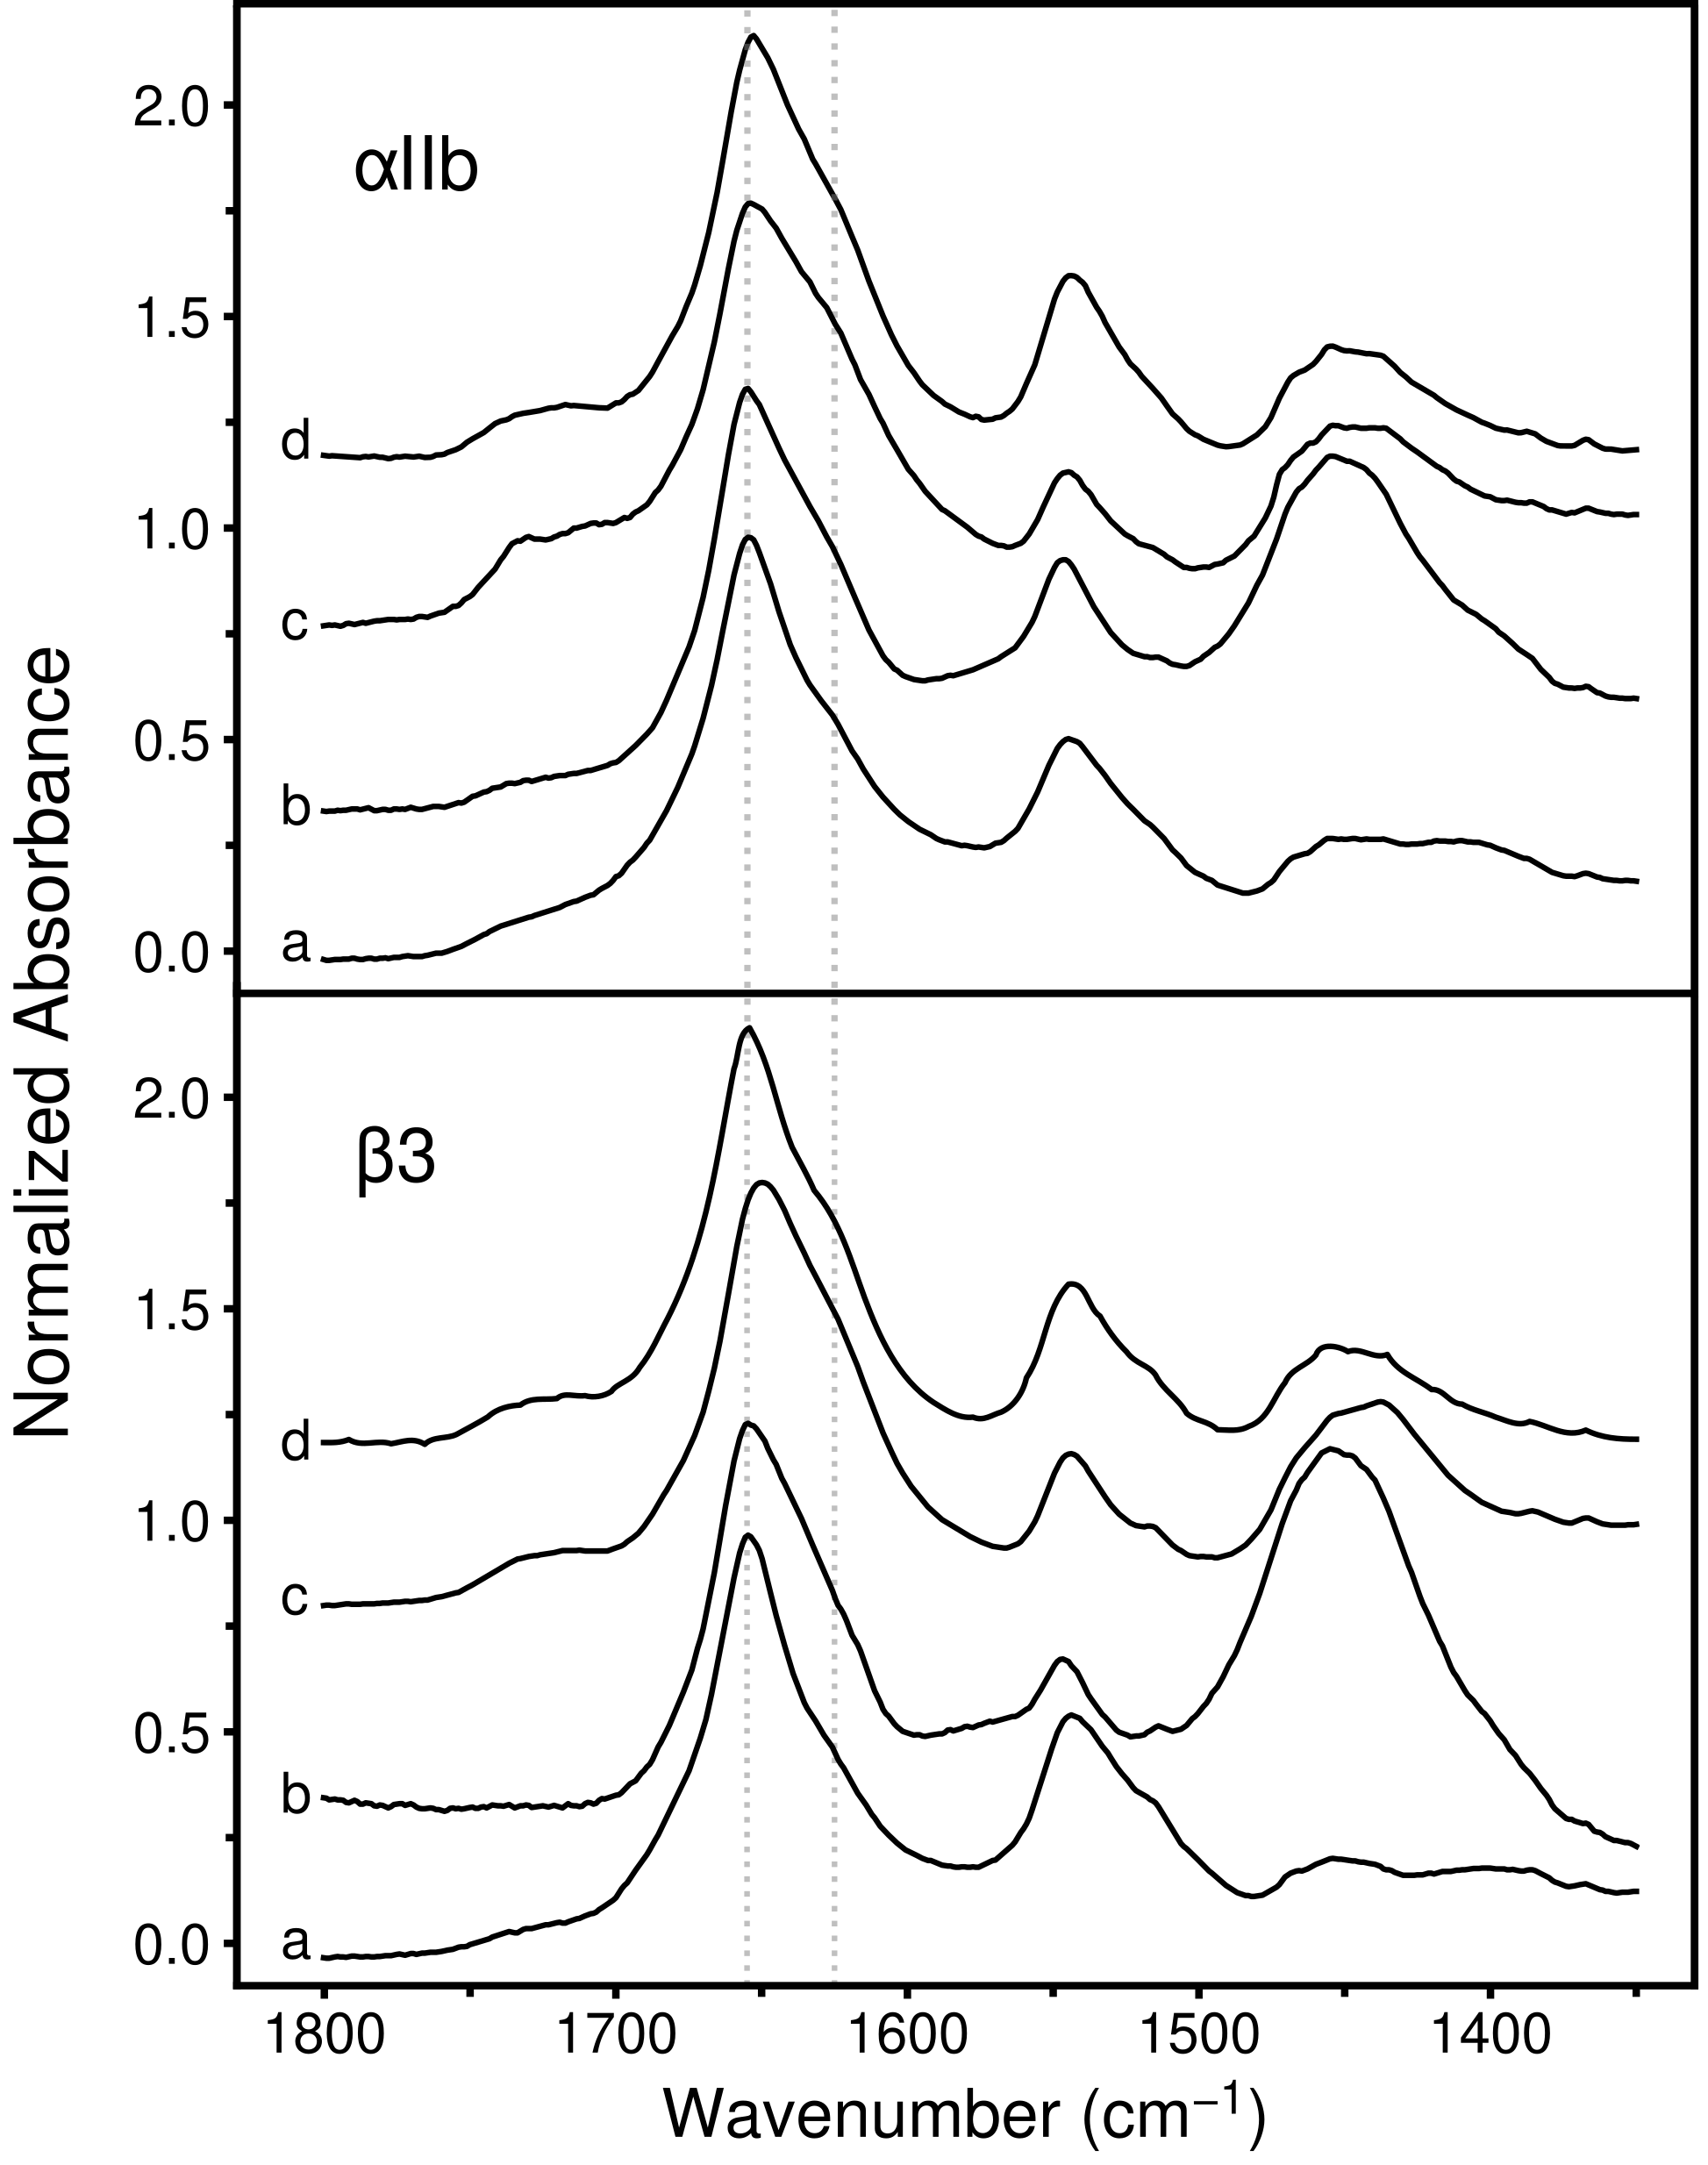
\includegraphics[width=0.4\linewidth, keepaspectratio]{fig1.png}
\caption{FTIR spectra of $\alpha$IIb peptides. Spectra \textbf{a}: samples dried from acetonitrile:water over the ATR crystal; spectra \textbf{b}: peptides dried over the ATR crystal from acetonitrile:water, rehydrated with D$_2$O in the crystal and further dried; spectra \textbf{c}: peptides dried outside the ATR crystal from acetonitrile:water, resuspended in D$_2$O and further dried over the ATR crystal;  spectra \textbf{d}: peptides dried outside the ATR crystal from acetonitrile:water, dissolved in chloroform:methanol, resuspended in D$_2$O and dried on the ATR crystal (See \hyperref[sec:expeSection]{Experimental Section}). Spectra were arbitrarily shifted in the ordinates axis. Dotted lines are traced at 1653 and 1626 cm$^{-1}$ for guiding the eye.}
\label{fig:ftir}
\end{figure}
%%%%%%%%%%% End %%%%%%%%%%%%

Fourier self deconvolution (FSD, see supporting information) revealed bands assigned to $\alpha$–helix and $\beta$ strands.\cite{1986_Byler} The spectra of samples directly dried from acetonitrile (traces \textbf{a} in \autoref{fig:ftir}) showed bands a 1655 cm$^{-1}$ corresponding to $\alpha$–helix, and at 1630 and 1679 cm$^{-1}$ corresponding to  $\beta$ strands. Bands at about the same position plus an extra band at 1615–1622 cm$^{-1}$ corresponding to  $\beta$ edges\cite{2003_Nolan} were observed for the samples that were in contact with D$_2$O (traces \textbf{b}, \textbf{c} and \textbf{d} in \autoref{fig:ftir}). Fitting of the component bands to the experimental spectra can provide an estimation of the proportion of secondary structure elements, although their fractional area not necessarily represent the actual proportion as determined, for example, by crystallography (see for example the results and discussions in Decca et al.\cite{2019_Decca}). In the samples dried directly from acetonitrile (traces \textbf{a} in \autoref{fig:ftir}) the band corresponding to $\alpha$–helix occupied about 55\% of the area of the amide I band, in the samples that were in contact with D$_2$O (traces \textbf{b}, \textbf{c} and \textbf{d} in \autoref{fig:ftir}), the band fitting resulted in about 44\% of the area for the $\alpha$–helix band (see \hyperref[sec:support]{Supplementary Table S1}). In spite of the lower area for the band at 1655 cm$^{-1}$ obtained by band fitting the spectral shape correspond to structures rich in $\alpha$–helix component, suggesting a tendency of both peptides to acquire this structure.\\


\noindent \textit{Peptide Structure Analysis}. 
We evaluated some properties of the peptides in the $\alpha$–helix conformation. \autoref{fig:mapHydrophob} shows the surface hydrophobicity of peptide $\alpha$IIb and peptide $\beta$3. Polar regions are segregated preferentially in the IC segments in both peptides. The IC, C terminal domain of peptide $\alpha$IIb contains five glutamic and two aspartic acids, two arginines and one lysine, the EC, N terminal domain contains two glutamic acids and one arginine. 
The IC segment of peptide $\alpha$IIb contains five glutamic and two aspartic acids, two arginines and one lysine, the EC, segment contains two glutamic acids and one arginine. The IC segment of peptide $\beta$3 contains fifteen ionizable residues: four arginines, four lysines, five glutamic and two aspartic acids, the EC segment contains one aspartic acid and one lysine (\hyperref[sec:support]{Supplementary Figure S2}A).

 The distribution of polar residues suggest that the peptides were preferentially oriented in the monolayer with the  EC and N terminal domains pointing towards the gas phase while the IC and C terminal domains  were preferentially interacting with the aqueous subphase.

%%%%%%%%%%% Figure %%%%%%%%%%%%
\begin{figure}
\centering
\includegraphics[width=0.3\linewidth, keepaspectratio]{fig2.png}
\caption{Surface hydrophobicity of the $\alpha$IIb$\beta$3 dimer.
Orange and blue portions represent the most hydrophobic and hydrophilic residues, respectively.}
\label{fig:mapHydrophob}
\end{figure}
%%%%%%%%%%% End %%%%%%%%%%%%

\autoref{fig:projHydropho} shows the helical wheel for the different segments of peptides $\alpha$IIb and $\beta$3 highlighting the hydrophobic character of the residues. The hydrophobic index <$H$> \cite{Eisenberg1982} and the hydrophobic moment (<$\mu_H$>)\cite{Eisenberg1982} of the segments with $N$ residues were calculated according to:  <$H$> $=  \frac{1}{N} \mathlarger{\Sigma}_{n=1}^NH_n $ and  <$\mu_H$> $= \frac{1}{N} \left(\left(\mathlarger{\Sigma}_{n=1}^{N}H_n \sin \text{(}\delta n\text{)} \right)^{2}+\left(\mathlarger{\Sigma}_{n=1}^{N} H_n \cos\text{(}\delta n\text{)}\right)^{2}\right)^{\frac{1}{2}}$, respectively.
As expected, the TM segments have a large hydrophobic index and a low hydrophobic moment, indicating that the TM segment are symmetric regarding the distribution of hydrophobic residues. The short EC segments and the large IC segments instead, are hydrophilic and have larger hydrophobic moment, characteristic of the amphipathic helix. The average hydrophobicities, hydrophobic moments and the net charge at pH 7 are shown in \autoref{tab:percent_hidrofo}. The low hydrophobicity of the IC segments, together with the net electric charge, supports the proposal that they are in contact with the water phase in the monolayer.\\


%%%%%%%%%%%% Figure %%%%%%%%%%%%
\begin{figure}[ht]
\centering
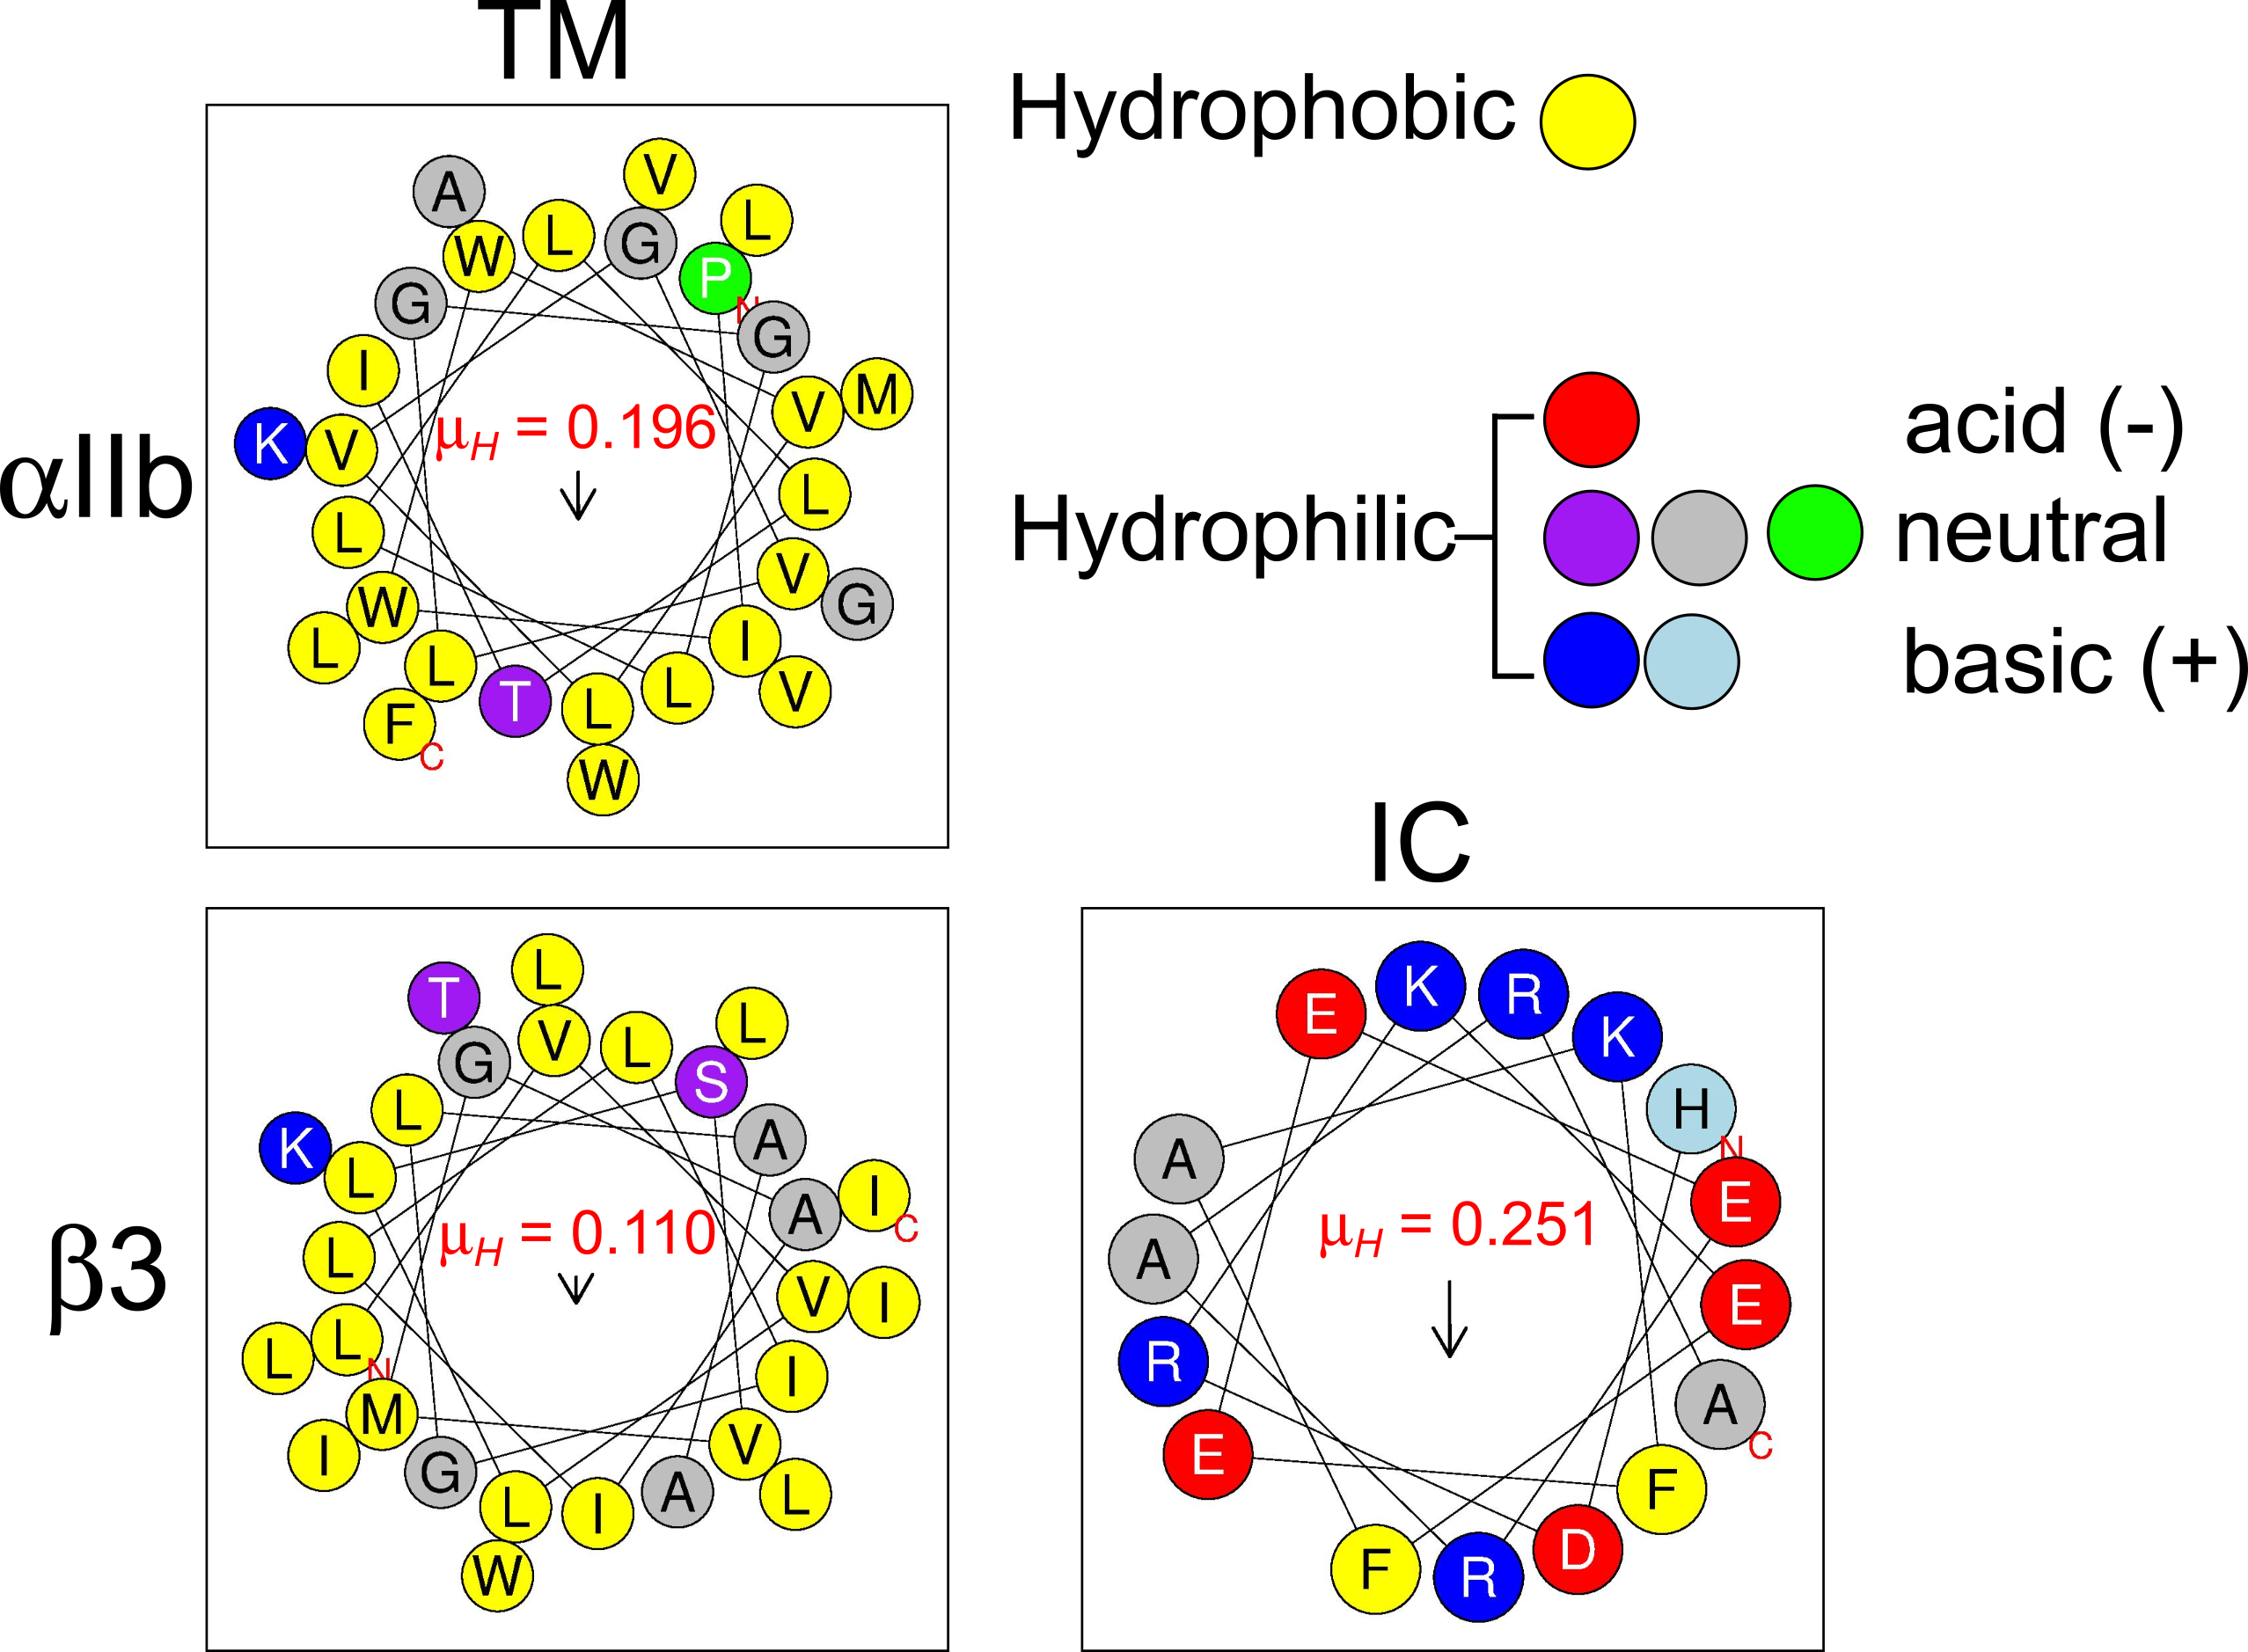
\includegraphics[width=0.4\linewidth, height=\textheight, keepaspectratio]{fig3.png}
\caption{Schiffer–Edmundson wheel projections of the $\alpha$IIb and $\beta$3 peptides. Color coding (HeliQuest): hydrophobic (Val, Leu, Met, Trp, Phe, Ile) in yellow; acidic (Glu, Asp) in red; polar uncharged (Ser, Thr) in purple; small neutral (Ala, Gly) in gray; Pro in green; basic (Lys, Arg) in blue; His in light blue. The arrow represents the mean hydrophobic moment vector, with direction and length indicating orientation and magnitude, respectively, toward the helix’s hydrophobic face.}
\label{fig:projHydropho}
\end{figure}
%%%%%%%%%%%% End %%%%%%%%%%%%


%%%%%%%%%%% Table %%%%%%%%%%%%
\begin{table}
\centering
\caption{Hydrophobicity (<H>) and hydrophobic moments (<$\mu_H$>) of $\alpha$–helix segments and net charge of all segments $\alpha$IIb and $\beta$3.}\label{tab:percent_hidrofo}
\begin{tabular}{@{}llccl@{}}
\toprule
Peptide     & Residues             & <H>       & <$\mu_H$> 	& z  \\ \midrule
$\alpha$IIb & \multirow{2}{*}{1–10 \; (EC)}      & –  	     & – 		    & 1– \\
$\beta$3    &                                    & –  	     & –            & 0  \vspace{3mm} \\

$\alpha$IIb & \multirow{2}{*}{11–38 \;(TM)}     & 1.182  	& 0.196 		& 1+ \\
$\beta$3    &                                   & 1.183  	& 0.110 		& 1+ \vspace{3mm} \\

$\alpha$IIb & \multirow{2}{*}{39–54 \;(IC)}     & – 	    & –		          & 4- \\
$\beta$3    &                                   & -0.231 	& 0.251 		    & 0  \vspace{3mm} \\

$\beta$3    & 55–79 \;(IC)                      & –  	& – 		& 1+ \\ \bottomrule
\end{tabular}
\end{table}
%%%%%%%%%%% End %%%%%%%%%%%%


\noindent \textit{Langmuir Monolayers. 
Lateral Stability of $\alpha$IIb and $\beta$3 Films}. An important consideration in the monolayer experimental approach is whether the surfactant remains in the interface or partitions, to some extent, into the subphase. Phospholipids, some glycolipids and long chain fatty acids, remain in the interface because of their amphiphilicity and low solubility in water. Besides, the measured area per molecule at the collapse surface pressure agrees with the geometry of these molecules \cite{1966_Gaines} indicating that all the material remains in the interface. This picture is not so Straightforward for other molecules like peptides or proteins. In this section we discuss the possible partition of the peptides considering the experimental results. \autoref{fig:potencialDipo} shows the behaviour of monolayers of pure peptides. The plots of surface pressure as a function of the molecular area (\autoref{fig:potencialDipo}A) were identical after three cycles of compression up to 5 mN$\cdot$m$^{-1}$ below the collapse surface pressure and decompression, indicating that the monolayers were stable. We cannot rule out that the peptides partitioned, to some extent, into the subphase when they were spread, but no further partitioning occurred as a consequence of the compression. Spreading 0.5 nmoles of peptide $\alpha$IIb or peptide $\beta$3 in a 75 cm$^2$ surface, corresponding to 2490 Å$^2$ per molecule, produced no increase in the surface pressure (\autoref{fig:potencialDipo}A) but did produce a large increase in the surface potential: 200 mV for peptide $\alpha$IIb and 150 mV for peptide $\beta$3, positive towards the air (\autoref{fig:mapHydrophob}B).  Upon compression, both peptides showed expanded monolayers and further increase in the surface potential. In our system, the peptide monolayers did not reach a neat and clear collapse. The mean molecular areas reached at 35 mN$\cdot$m$^{-1}$ were 587 $\pm$ 25 Å$^2$ and 488 $\pm$ 25 Å$^2$ for $\alpha$IIb and  $\beta$3, respectively. The average cross sectional area of the peptides, obtained from the PDB structure (PDB ID 2KNC), are 117 Å$^2$ for peptide $\alpha$IIb and 137 Å$^2$ for $\beta$3. 
The comparison with the experimental values suggests that at the maximal surface pressure reached the peptides were not closely packed as vertical, dehydrated $\alpha$-helix. It can be supposed that several configurations were present, like vertical, tilted, horizontal and surrounded by structured water. The IC, C terminal domain of the peptide $\beta$3 is larger than the corresponding segment of the peptide $\alpha$IIb. 
Nevertheless, the molecular areas at a given surface pressure along the isotherms, particularly at the highest surface pressure, were similar. This suggests that the IC segment of $\beta$3 was located most probably in the aqueous environment and acquired an $\alpha$-helix conformation along the whole isotherm.


%%%%%%%%%%%% Figure %%%%%%%%%%%%
\begin{figure}[ht]
\centering
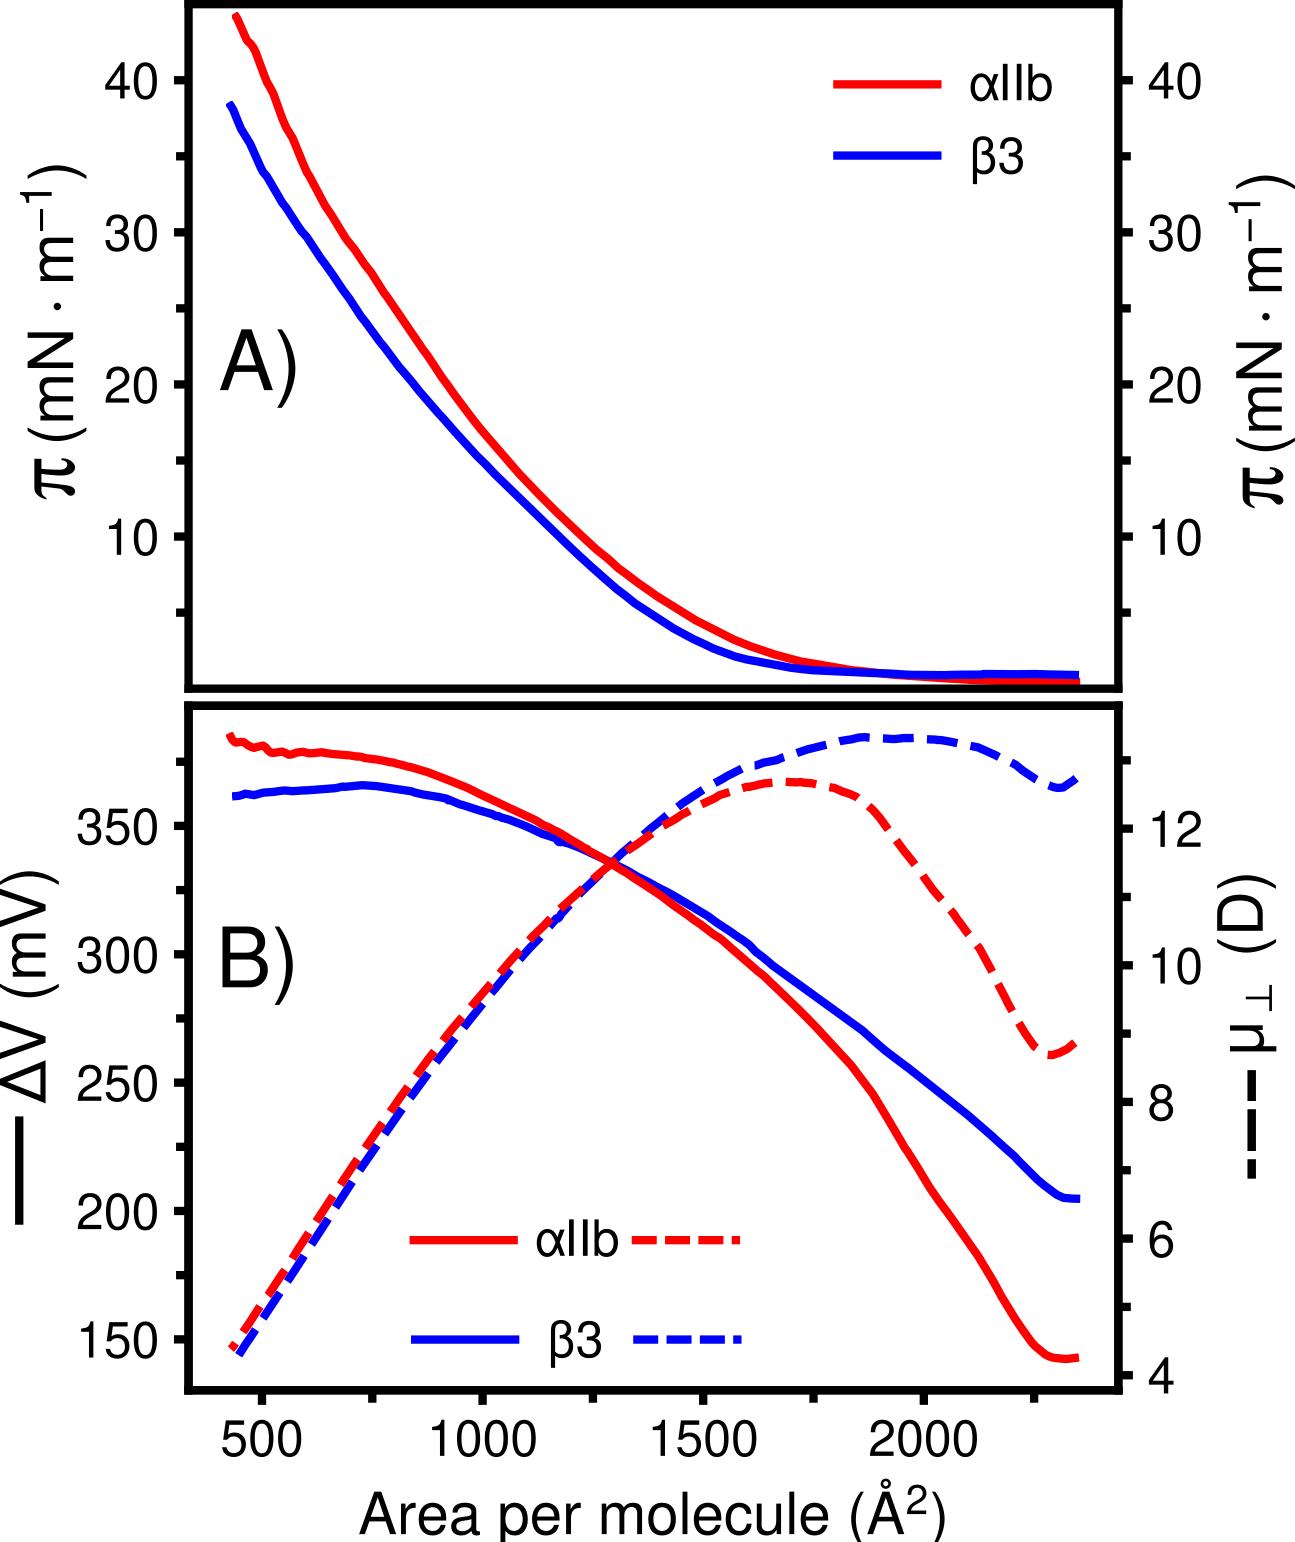
\includegraphics[width=0.4\linewidth, height=\textheight, keepaspectratio]{fig4.png}
\caption{ Surface behaviour of $\alpha$IIb and $\beta$3. A) surface pressure ($\pi$), B) surface potential ($\Delta$V, \textbf{–}) and perpendicular component of surface dipole ($\mu_\perp$, \textbf{- - -}) as a function of the mean molecular area.}
\label{fig:potencialDipo}
\end{figure}
%%%%%%%%%%%% End %%%%%%%%%%%%

Already at very low surface pressures, actually indistinguishable from zero, both peptides induced a large surface potential with the air positive with respect to the aqueous phase. The compression of the monolayer produced further increase in the surface potential to reach values of 310 mV for peptide $\alpha$IIb and 375 mV for peptide $\beta$3.
 It must be noted that while the slope of the surface potential curves changed to reach approximately constant values at small areas, between 500 and 1000 Å$^2$, the pressure was still increasing upon compression. This means that the molecular reorganization that occurred upon compression did not have an effect on the surface potential. Our interpretation is that the surface potential had a large contribution from the macroscopic, global arrangement of the monolayer rather than molecular ordering of the dipoles of the peptides. By global arrangements, we refer to the ordering of interfacial water in contact with peptides and changes in the electrical permitivity of the interface (see below). We propose that interfacial water was already ordered, at low surface pressure, when the peptides were still able to further reorganize upon compression.\\

\noindent \textit{Surface Potential of Pure Peptides}. 
The electric surface potential is directly related to the dipolar  organization of the monolayer. According to the Helmholtz equation \cite{Brockman1994} the surface potential is proportional to the normal component of the surface dipole: $\Delta V =  \frac{12 \Pi \mu_\perp}{A}$.  $\Delta V$ is in mV, the molecular area \textit{A} is in Å$^2$, and the dipole moment $\mu_\perp$ is in mD. 

The evaluation of the vertical component, $\mu_\perp$, of the macroscopic dipole can give us information about the structure and molecular organization of the monolayer. The vertical component of the surface dipole moment $\mu_\perp$ is expressed as mD per molecule. As discussed in the papers by Vogel et al.\cite{Vogel1988} and by Taylor \cite{Taylor1994}, $\mu_\perp$ is not due only to the the dipole moment of the spread molecules. Three components contribute to $\mu_\perp$: the Gouy–Chapman double layer, the orientationaly and/or electronic polarized water in the interface and the the vertical component of the dipole moment of the adsorbed molecules. \cite{Brockman1994}. We obtained total surface dipoles with the positive end pointing towards the gas phase (\autoref{fig:potencialDipo}B). If we consider that at large surface areas, low $\pi$, both peptides are oriented parallel to the surface, the dipole of the $\alpha$–helix backbone should not contribute to the dipole vertical component. The monolayer of peptide $\beta$3 produced a positive surface potential, consistent with a Gouy–Chapman double layer generated by positive amino acids. The peptide $\alpha$IIb, supporting a negative charge, also produced a positive surface potential and positive $\mu_\perp$. Upon compression, the surface dipole showed a bimodal behaviour. For the peptide $\alpha$IIb, $\mu_\perp$ slightly increased and then decreased, for the peptide $\beta$3 the first increase of $\mu_\perp$ was larger an then also decreased (\autoref{fig:potencialDipo}B). 

Between 1700 and 500 Å$^2$, both curves were coincident. Considering the large difference of net charge distribution in peptide $\alpha$IIb and peptide $\beta$3, it is difficult to attribute the similarity of $\mu_\perp$ values to particular molecular orientations and conformations. We propose instead that the surface potential and calculated $\mu_\perp$ values are due to global, unspecific properties of the interface like water orientations or changes in the monolayer permittivity.\\


\noindent \textit{Lipid–Peptide Interactions}. 
We studied monolayers of mixed films to know about the interactions of peptide $\alpha$IIb and peptide $\beta$3 with lipids. Two main properties of lipid monolayer, as a first approach, were considered to have an influence on the interactions with the peptides: the phase state and the electric charge. We used a zwitterionic lipid in the LE phase, POPC, and a zwitterionic lipid that undergoes a phase transition between LE and LC phase, DPPC. To study the influence of electric charge we used a mixture of a zwitterionic and an anionic lipid in the LE phase, POPC:POPG 70:30 (PC–PG). This proportion was chosen arbitrarily to produce a negatively charged interface, but not a strong, non–physiological electrostatic force as could be a 100\% anionic lipid monolayer. It must be noted that the chosen proportion is about twice the proportion of anionic charges in a platelet plasma membrane \cite{1996_Garcia}.


\autoref{fig:mixIsothe} shows the compression isotherms of the pure lipids and the different mixtures with peptides $\alpha$IIb and $\beta$3. Both peptides produced an expansion of the monolayers of the zwitterionic lipids POPC and DPPC but not in the amount expected for an ideal mixture (see below). Mixtures with POPC and with PC–PG had smaller areas than expected for an ideal mixing. Mixtures with DPPC reached larger areas instead. A major effect of both peptides  was a marked reduction in the DPPC phase transition, observable even at low peptide proportions. In the presence of peptides DPPC was in the LE phase as concluded from the shape of the isotherm and the compressibility (see below \autoref{fig:Cs1}).



The anionic mixture PC–PG showed a bimodal behavior. Peptide $\alpha$IIb produced a small expansion at 2.0\% and 3.5\% peptide, a compression of the monolayer at 5.0\% and a small compression at 7.0\%. The effect was more noticeable with peptide $\beta$3: almost no change in the isotherm was produced with 2.0\% peptide, a remarkable compression occurred at 3.5\% and 5.0\% peptide and at 7.0\% peptide the isotherm was again similar to the pure lipid (see Figure 5). If we take into account that they have opposite electric net charge, 4$^{-}$ for $\alpha$IIb and 2$^{+}$ for $\beta$3, we realize that it is not a simple effect of attraction or repulsion between peptides and lipids. The electrostatic attractions between peptide $\beta$3 and the negatively charged lipid could produce peptide–lipid complexes with lower area per lipid, accounting for the decrease in area. Nevertheless, the anionic peptide $\alpha$IIb produced a similar effect. This can be explained if we take into account that peptides and lipids are not rigid bodies, they have a large conformational space and can explore many conformations and locations in the interface. For the case of peptide $\alpha$IIb we can propose that the peptide–lipid repulsion due to negative charges could slide the peptide out of the plane of the monolayer generating arrangements of lower area per molecule.


%%%%%%%%%%%% Figure %%%%%%%%%%%%
\begin{figure}[ht!]
\centering
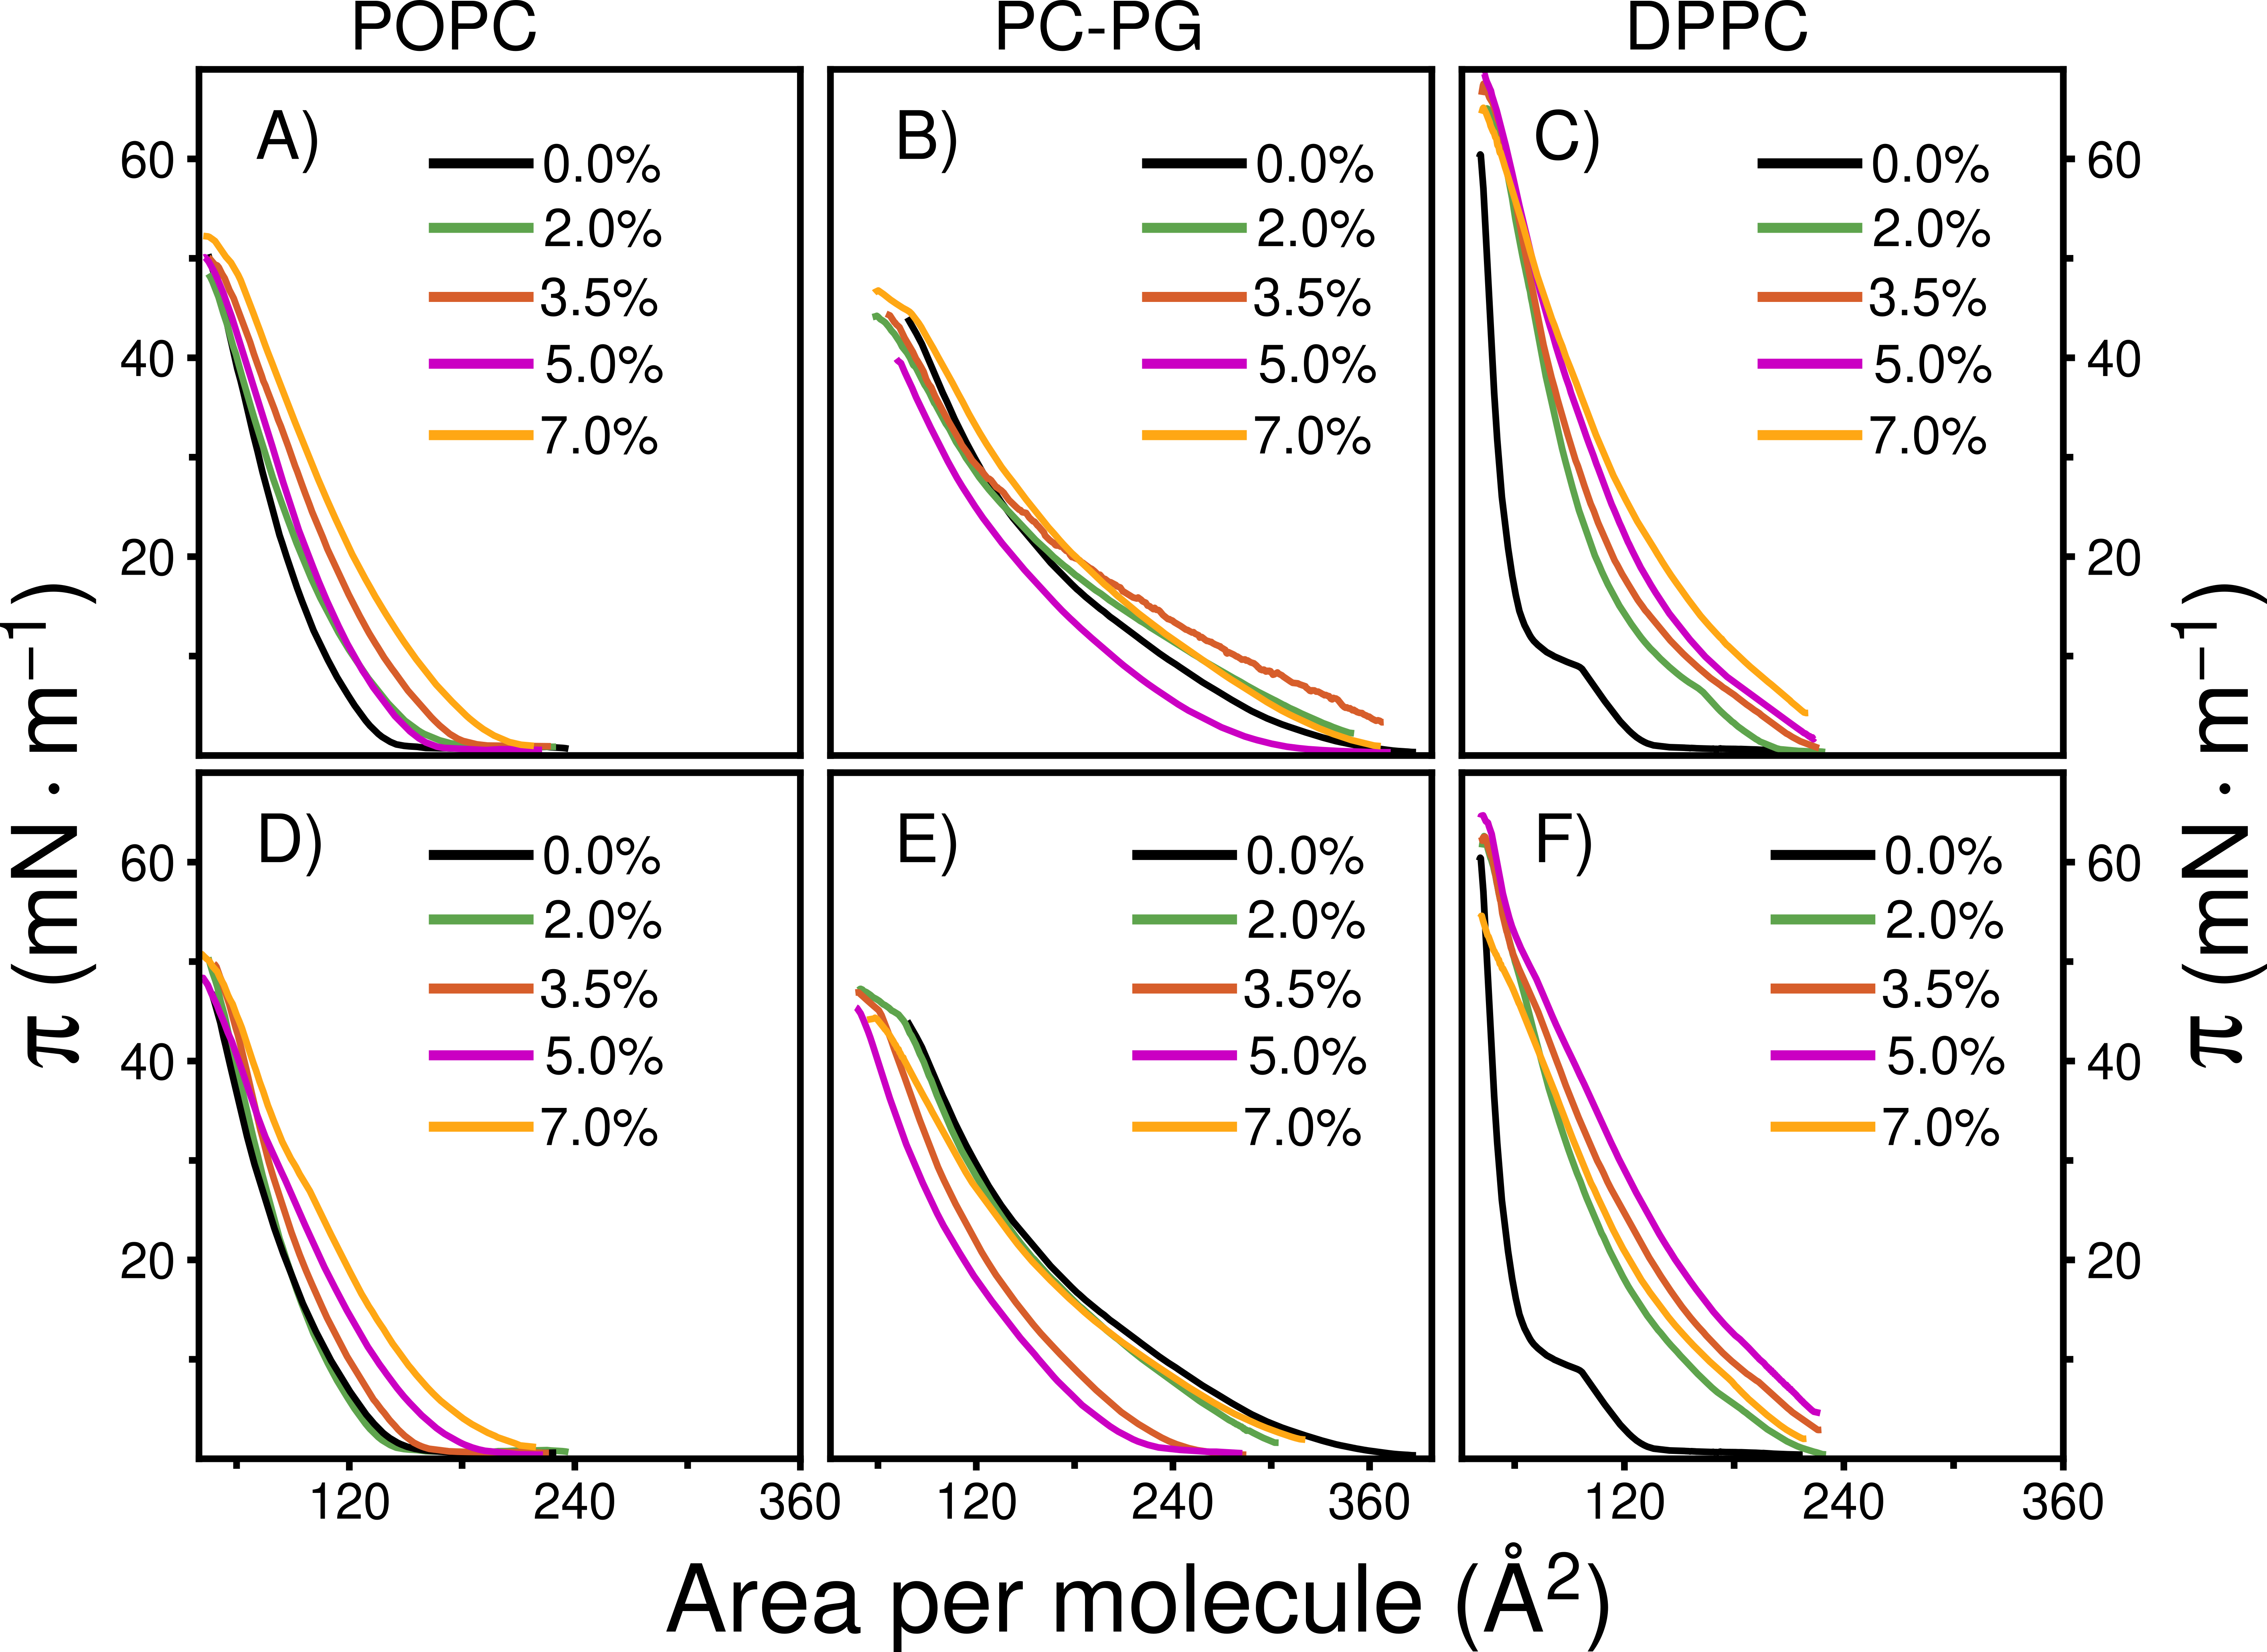
\includegraphics[width=0.7\linewidth, height=\textheight, keepaspectratio]{fig5.png}
\caption{Surface pressure–area compression isotherms ($\pi$–A) for pure lipids films and their mixtures with peptides. A-C) mixtures lipid–$\alpha$IIb, D-F) mixtures lipid–$\beta$3. Each curve represents the average of at least three independent measurements. Peptide mole fractions are represented by lines with different colors.}
\label{fig:mixIsothe}
\end{figure}
%%%%%%%%%%%% End %%%%%%%%%%%%

Further understanding of the peptide–lipid interactions can be obtained evaluating the departure from the ideal mixing. The ideal area, $A_{ideal}$, at a given $\pi$ is calculated according to: $A_{ideal} = \left(X_{\textit{l}}A_{\textit{l}} + X_{\textit{p}}A_{\textit{p}}\right)_\pi$, where $X_{\textit{l}}$ and $X_{\textit{p}}$ are the mole fractions and $A_{\textit{l}}$ and $A_{\textit{p}}$ are the molecular areas of the pure components, the index \textit{l} and \textit{p} are for lipid and peptide respectively.  \autoref{fig:areaIdealMix}, dashed lines, shows the areas expected for an ideal mixing.  These are the areas expected if the mixing occurred without interactions, or with compensating interactions. Symbols and lines show the actual areas obtained at 2 and 30 mN$\cdot$m$^{-1}$ of the different mixtures. For POPC we conclude that even when the peptide produced an expansion (isotherms located to the right of the pure lipid monolayer, \autoref{fig:mixIsothe}), it is not as large as expected for an ideal behaviour, both for peptides $\alpha$IIb and $\beta$3.


Mixed monolayers of peptides and DPPC displayed a different behaviour. The mixtures with peptide $\alpha$IIb, evaluated at 2 and 30 mN$\cdot$m$^{-1}$, were close to the ideal behaviour, with a small positive deviation at 2.0 mole\% and a small negative deviation at 7.0 mole\%. The mixtures of peptide $\beta$3 departed slightly more from ideality, positively between 2.0 and 5.0 mole\% and slightly negatively at 7.0 mole\% (\autoref{fig:areaIdealMix}).

%%%%%%%%%%%% Figure %%%%%%%%%%%%
\begin{figure}[hb!]
\centering
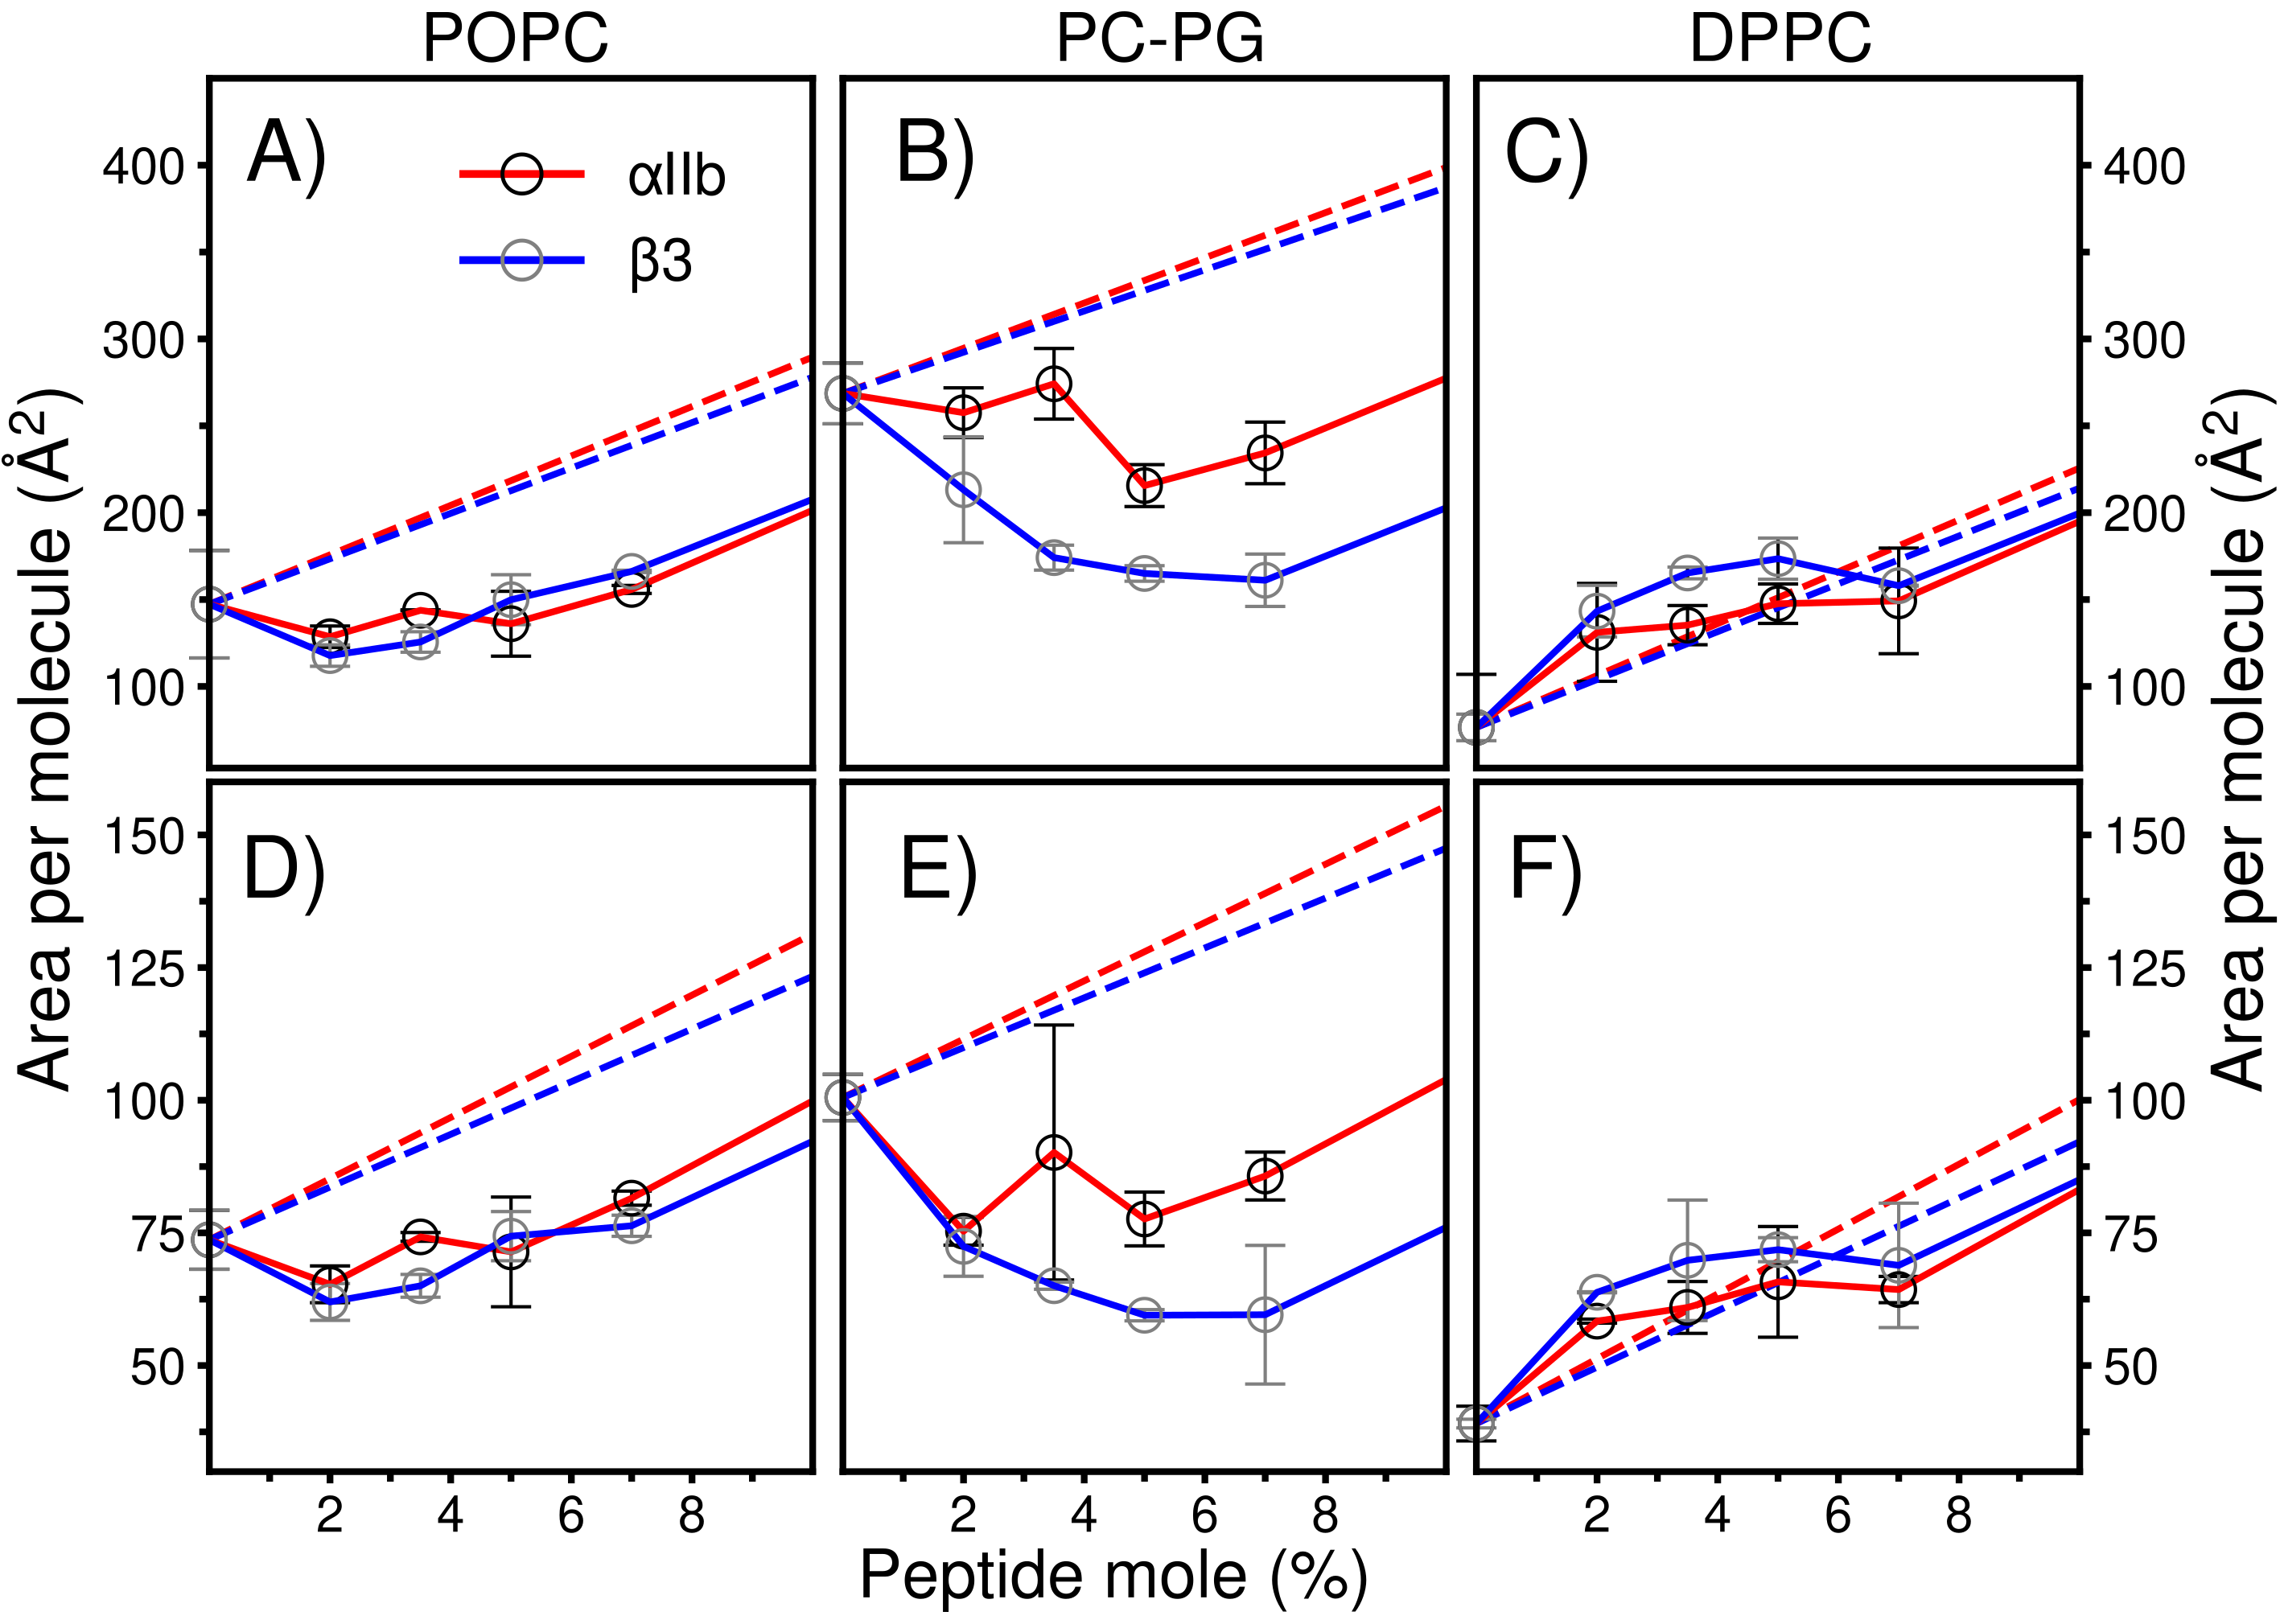
\includegraphics[width=0.6\linewidth, height=\textheight, keepaspectratio]{fig6.png}
\caption{Mean molecular areas as a function of the molar fraction of the peptide for the studied monolayers at different surface pressures: A-C) $\pi$=2 mN$\cdot$m$^{-1}$ and D-F) $\pi$=30 mN$\cdot$m$^{-1}$. The average value $\pm$ the standard deviation of at least 3 independent measurements are depicted. Dashed lines correspond to mean molecular area of an ideal mixture. Continuous lines and symbols correspond to the experimental molecular area.}
\label{fig:areaIdealMix}
\end{figure}
%%%%%%%%%%%% End %%%%%%%%%%%%

We observed a large negative deviation in the mixtures with the anionic monolayer. The cationic peptide $\beta$3 produced a greater decrease in areas compared to the peptide $\alpha$IIb, consistent with attractive interactions with anionic lipids. However, the anionic peptide $\alpha$IIb also produced a negative deviation, although smaller, which is also indicative of compression in the average molecular areas.
We also evaluated the deviation from ideal mixing using the approach introduced by Socas and Ambroggio \cite{Socas2018,Socas2023}. This method compares a given isotherm with a reference isotherm. The comparison is along the common values of molecular area and surface pressure. The parameter $\Lambda$ is defined by two numbers $\lambda$ and \textit{r}$^2$: $\Lambda = \left(\lambda,r^2 \right)$.

An isotherm is constructed by multiplying the isotherm of interest by $\lambda$. A non linear regression algorithm search for the $\lambda$ value that minimize the difference between the constructed isotherm and the reference isotherm. The determination coefficient \textit{r}$^2$ is obtained by comparison of the constructed isotherm with the reference isotherms. For two identical isotherms (same shape and location in the $\pi$–area curve), $\Lambda$ = (1, 1). For \textit{r}$^2$ = 1, isotherms more expanded than the reference have $\lambda$ > 1 and for more compact isotherms have $\lambda$ < 1. 
Values of \textit{r}$^2$ <\! 1 indicate that the isotherms are different in shapes. In this way, the comparison between isotherms is done along the whole range of surface pressures. 
We compared the experimental isotherms with the corresponding ideal mixing isotherms as the reference. \autoref{fig:lambda} shows the values of $\lambda$ and \textit{r}$^2$ for the different mixed monolayers. 
The values of $\lambda$ indicated that the mixtures of any of both peptides with POPC and with the anionic monolayer PC–PG resulted in molecular areas smaller than the ideal. Mixed monolayers with DPPC were close to the ideal mix for peptide $\alpha$IIb and with molecular areas larger than the ideal for peptide $\beta$3. 
The results of this analysis are in agreement with the classical treatment shown in \autoref{fig:areaIdealMix}. The values of \textit{r}$^2$ were close to one for POPC and PC–PG, indicating that the isotherms preserved a shape similar to the ideal isotherm. Values of  \textit{r}$^2$ lower than  \textit{r}$^2$ = 1, in the case of DPPC, indicated that the mixed monolayer had a different shape than the ideal, which is in agreement with the lack of the phase transition plateau of DPPC in the presence of peptides.


These results suggest that mixtures containing either the $\alpha$IIb or $\beta$3 peptide had a condensing effect on lipids in the LE phase ($\lambda$ < 1). Furthermore, the presence of a negative charge (from POPG) enhanced this condensation, as shown in \autoref{fig:areaIdealMix} and \autoref{fig:lambda}. Contrary, in mixtures with DPPC, the $\lambda$ values approached 1, and in some cases, $\lambda$ > 1, indicating expansive interactions between lipids and peptides.\\

%%%%%%%%%%%% Figure %%%%%%%%%%%%
\begin{figure}[h!]
\centering
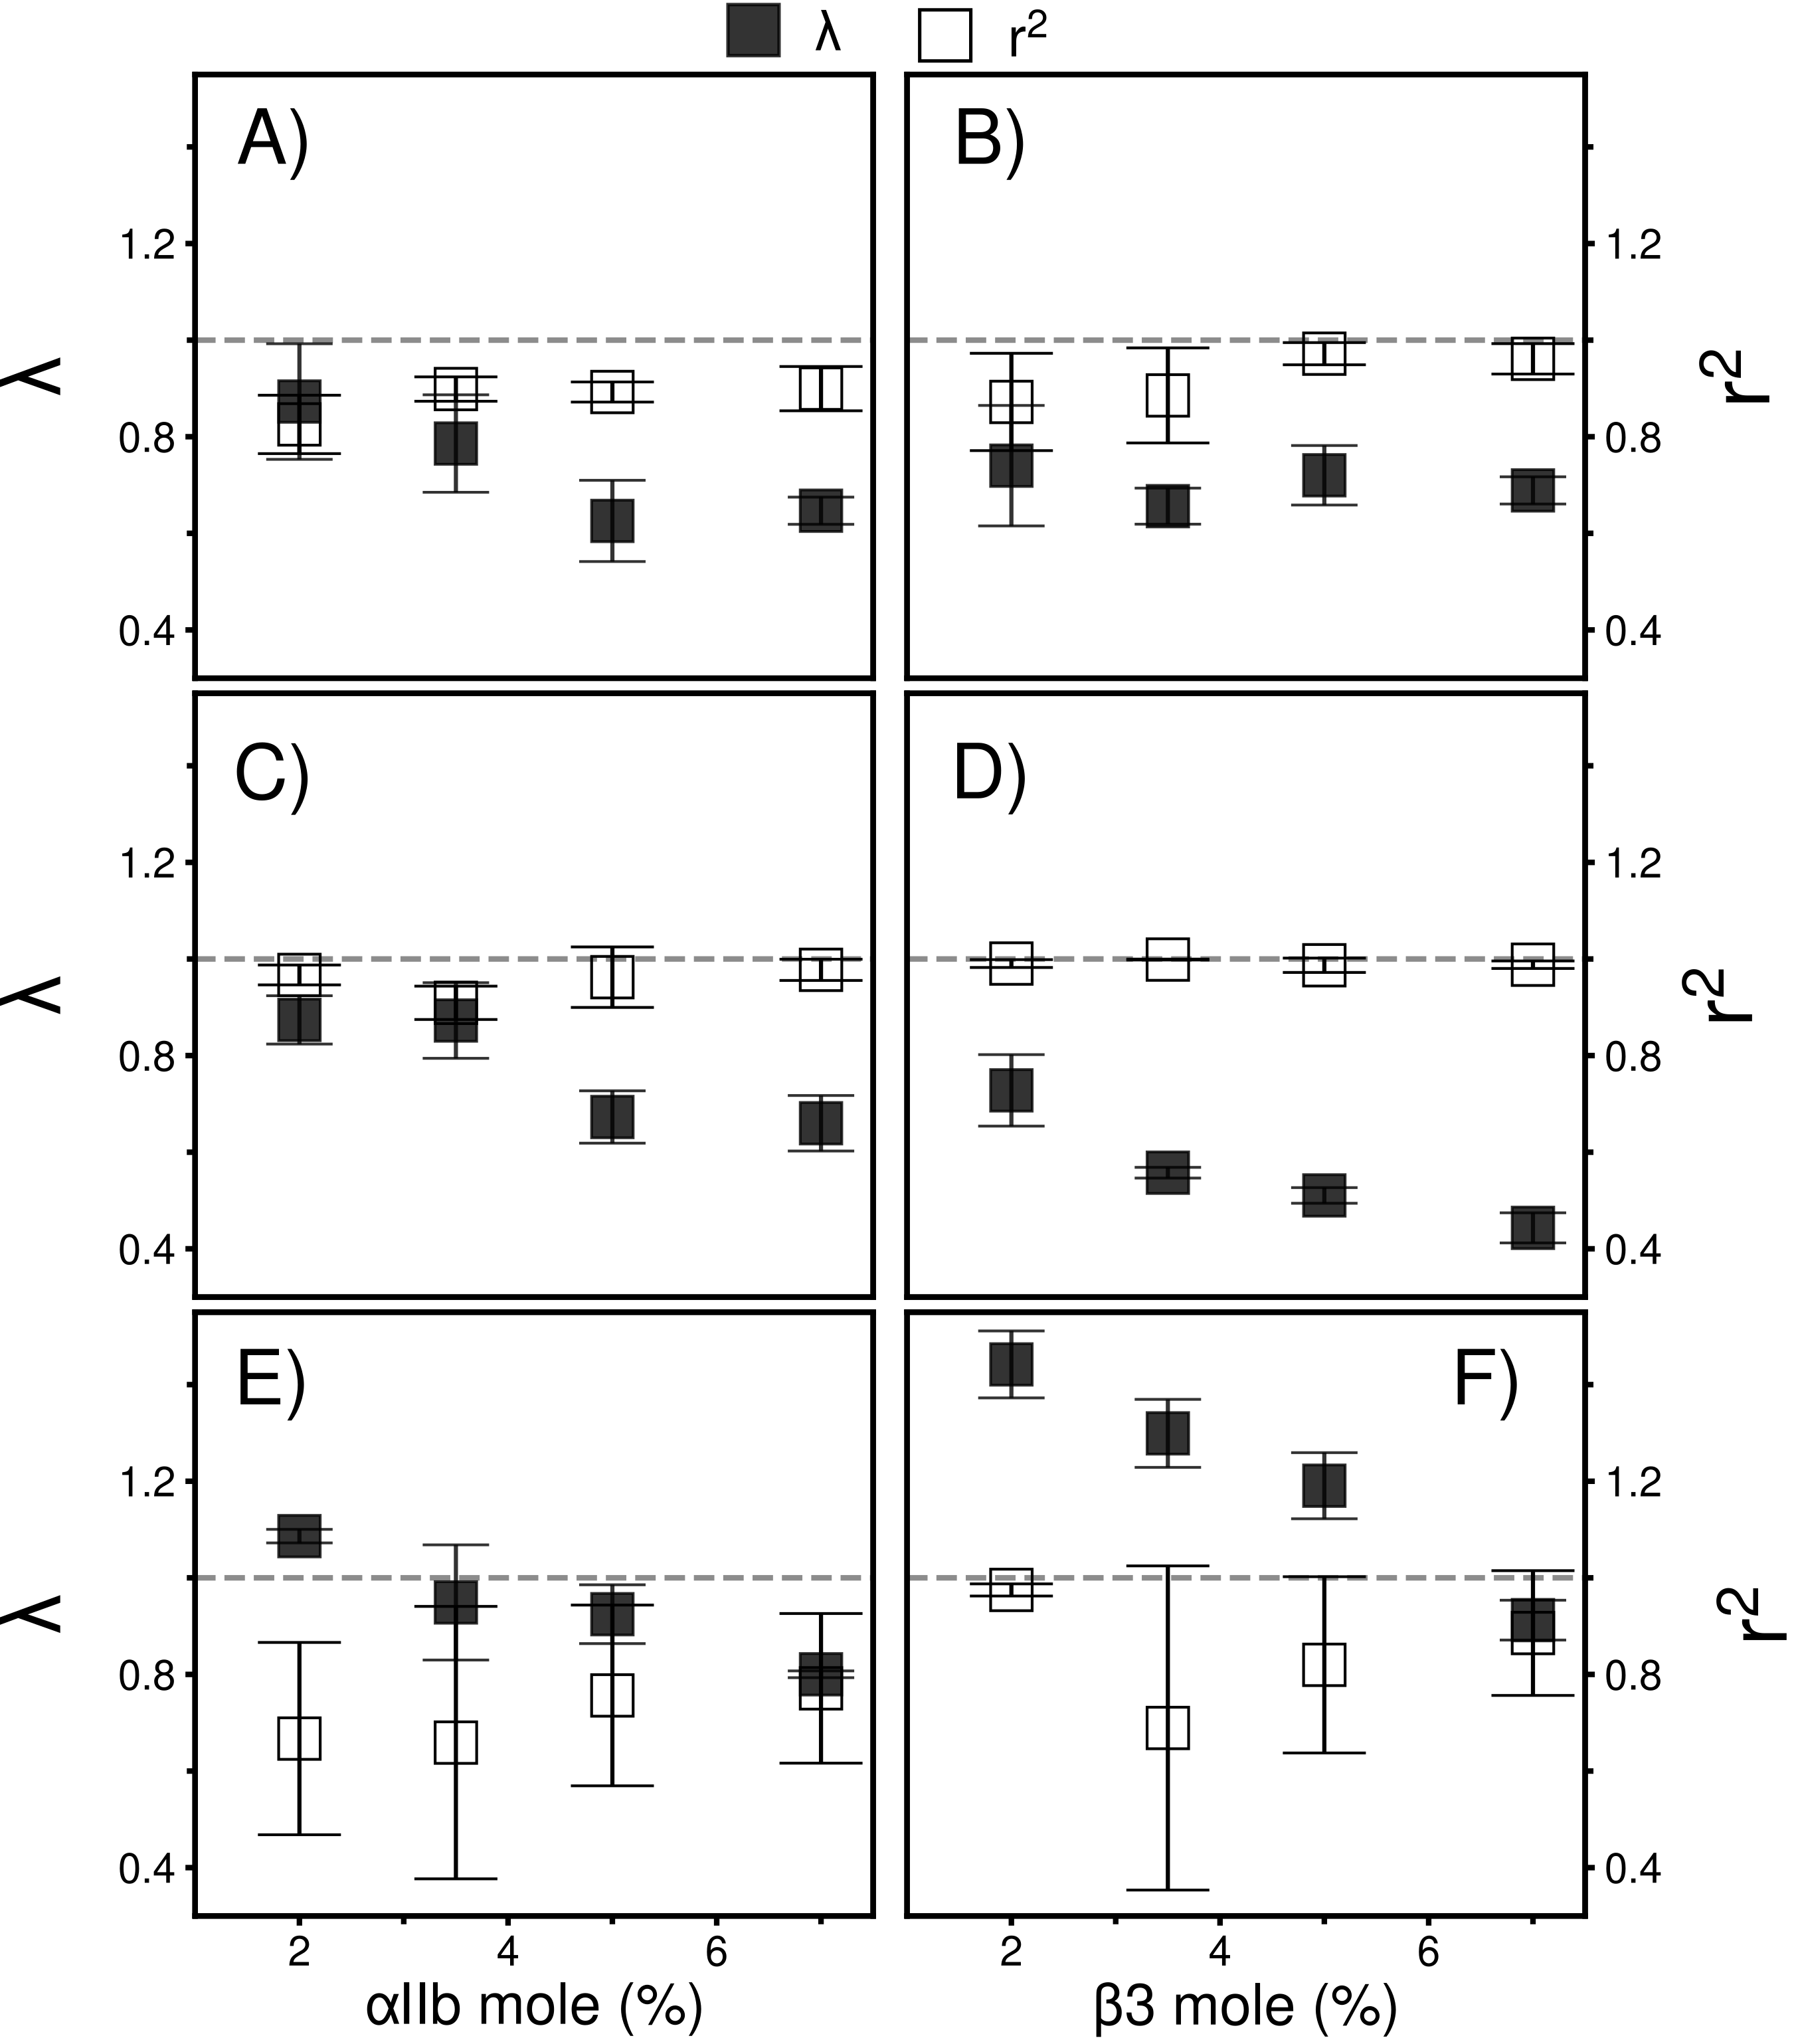
\includegraphics[width=0.5\linewidth, height=\textheight, keepaspectratio]{fig7.png}
\caption{Analysis of the  $\Lambda$–factor for lateral miscibility studies. Lipid interfaces A-B) POPC, C-D) PC–PG and E-F) DPPC with $\alpha$IIb  and $\beta$3 peptide. The values of $\lambda$ and \textit{r}$^2$ are shown for the comparison between the real and ideal compression isotherms of lipid interfaces as a function of the molar fraction of the peptide. The dashed line indicates the value of $\lambda$ = 1 as a reference of the ideal case.}
\label{fig:lambda}
\end{figure}
%%%%%%%%%%%% End %%%%%%%%%%%%

\noindent \textit{Surface Potential and Dipolar Organization of Pure Lipids and Mixed Monolayers}. 
In all cases, for pure lipids and their mixtures with peptides, the macroscopic surface potential increased with compression. The monolayers of pure lipids showed different dependences of the surface potential and vertical dipole with the molecular area. Surface potential of POPC increased with a relatively large slope between the start of the isotherm and 150 Å$^2$ (gas phase), and increased further with a smaller slope until collapse (LE). In the PC–PG mixture the $\Delta V$ increased monotonically upon compression without large differences between gas and LE phase, because it starts at 350 Å$^2$ due to electrostatic repulsion. In DPPC $\Delta V$ showed a complex dependence as a function of the molecular area following four regime: gas, LE, LE–LC, LC.\\

\noindent \textit{Mixtures of Lipids with $\alpha$IIb Peptide}. 
 In POPC at proportions 2.0, 3.5 and 5.0 mole\% the peptide $\alpha$IIb had no major influence on $\Delta V$ and $\mu_\perp$, at 7.0 mole\% produced an increase in $\Delta V$ and $\mu_\perp$ at low surface pressure (\autoref{fig:mu_dV_alfa}A,B). A bimodal behaviour as a function of peptide concentration was observed in PC–PG, a small increase in $\Delta V$ and $\mu_\perp$ was observed at low proportions, 2.0 and 3.5 mole\% and a small decrease at 5.0 and 7.0 mole\% (\autoref{fig:mu_dV_alfa}). In DPPC, $\alpha$IIb produced small increases in $\Delta V$ and $\mu_\perp$, the remarkable feature was that the differentiated regimes of pure DPPC were absent, also consistent with the elimination of the phase transition in the $\pi$–area curve (\autoref{fig:mu_dV_alfa}A,B).\\

\noindent \textit{Mixtures of Lipids with $\beta$3 Peptide}.
Similar general results as with peptide $\alpha$IIb were observed for peptide $\beta$3 with the particular differences that i) in POPC, the increases in $\Delta V$ and $\mu_\perp$ were already observed at 3.5 mole\% and that ii) a larger increase in $\Delta V$ and $\mu_\perp$ occurred in PC–PG at intermediate $\pi$–areas, that is in the range 150–200 Å$^2$ per molecule (\autoref{fig:mu_dV_alfa}A,B).

The peptides $\alpha$IIb and $\beta$3 have macro dipoles of different magnitude and net charges of opposite sign, nevertheless, both peptides produced about the same changes in the surface potential of lipid monolayers. Our interpretation is that these changes are due to nonspecific effects, mainly the organization of water in the interface. The ionic double layer produced by anionic lipids generates a partial dipole with the positive end pointing towards the water phase. Nevertheless, in the absence of peptides, the mixture PC–PG produced positive $\Delta V$ values, larger than pure POPC, indicating that other factors like the ordering of water and changes in dielectric constant of the interface have more influence on $\Delta V$ values.
Then, it is not surprising that the peptides produced changes in surface potential not directly predictable from their net charge: both peptides, with positive and negative net charge, produced positive surface potential. It must be noted that even when pure peptide $\beta$3 produced a smaller positive $\Delta V$ value than peptide $\alpha$IIb at low surface pressure (\autoref{fig:potencialDipo}), it was more efficient than $\alpha$IIb to shift the $\Delta V$ of pure POPC to larger positives values (\autoref{fig:mu_dV_alfa}).

%%%%%%%%%%%% Figure %%%%%%%%%%%%
\begin{figure}[h!]
\centering
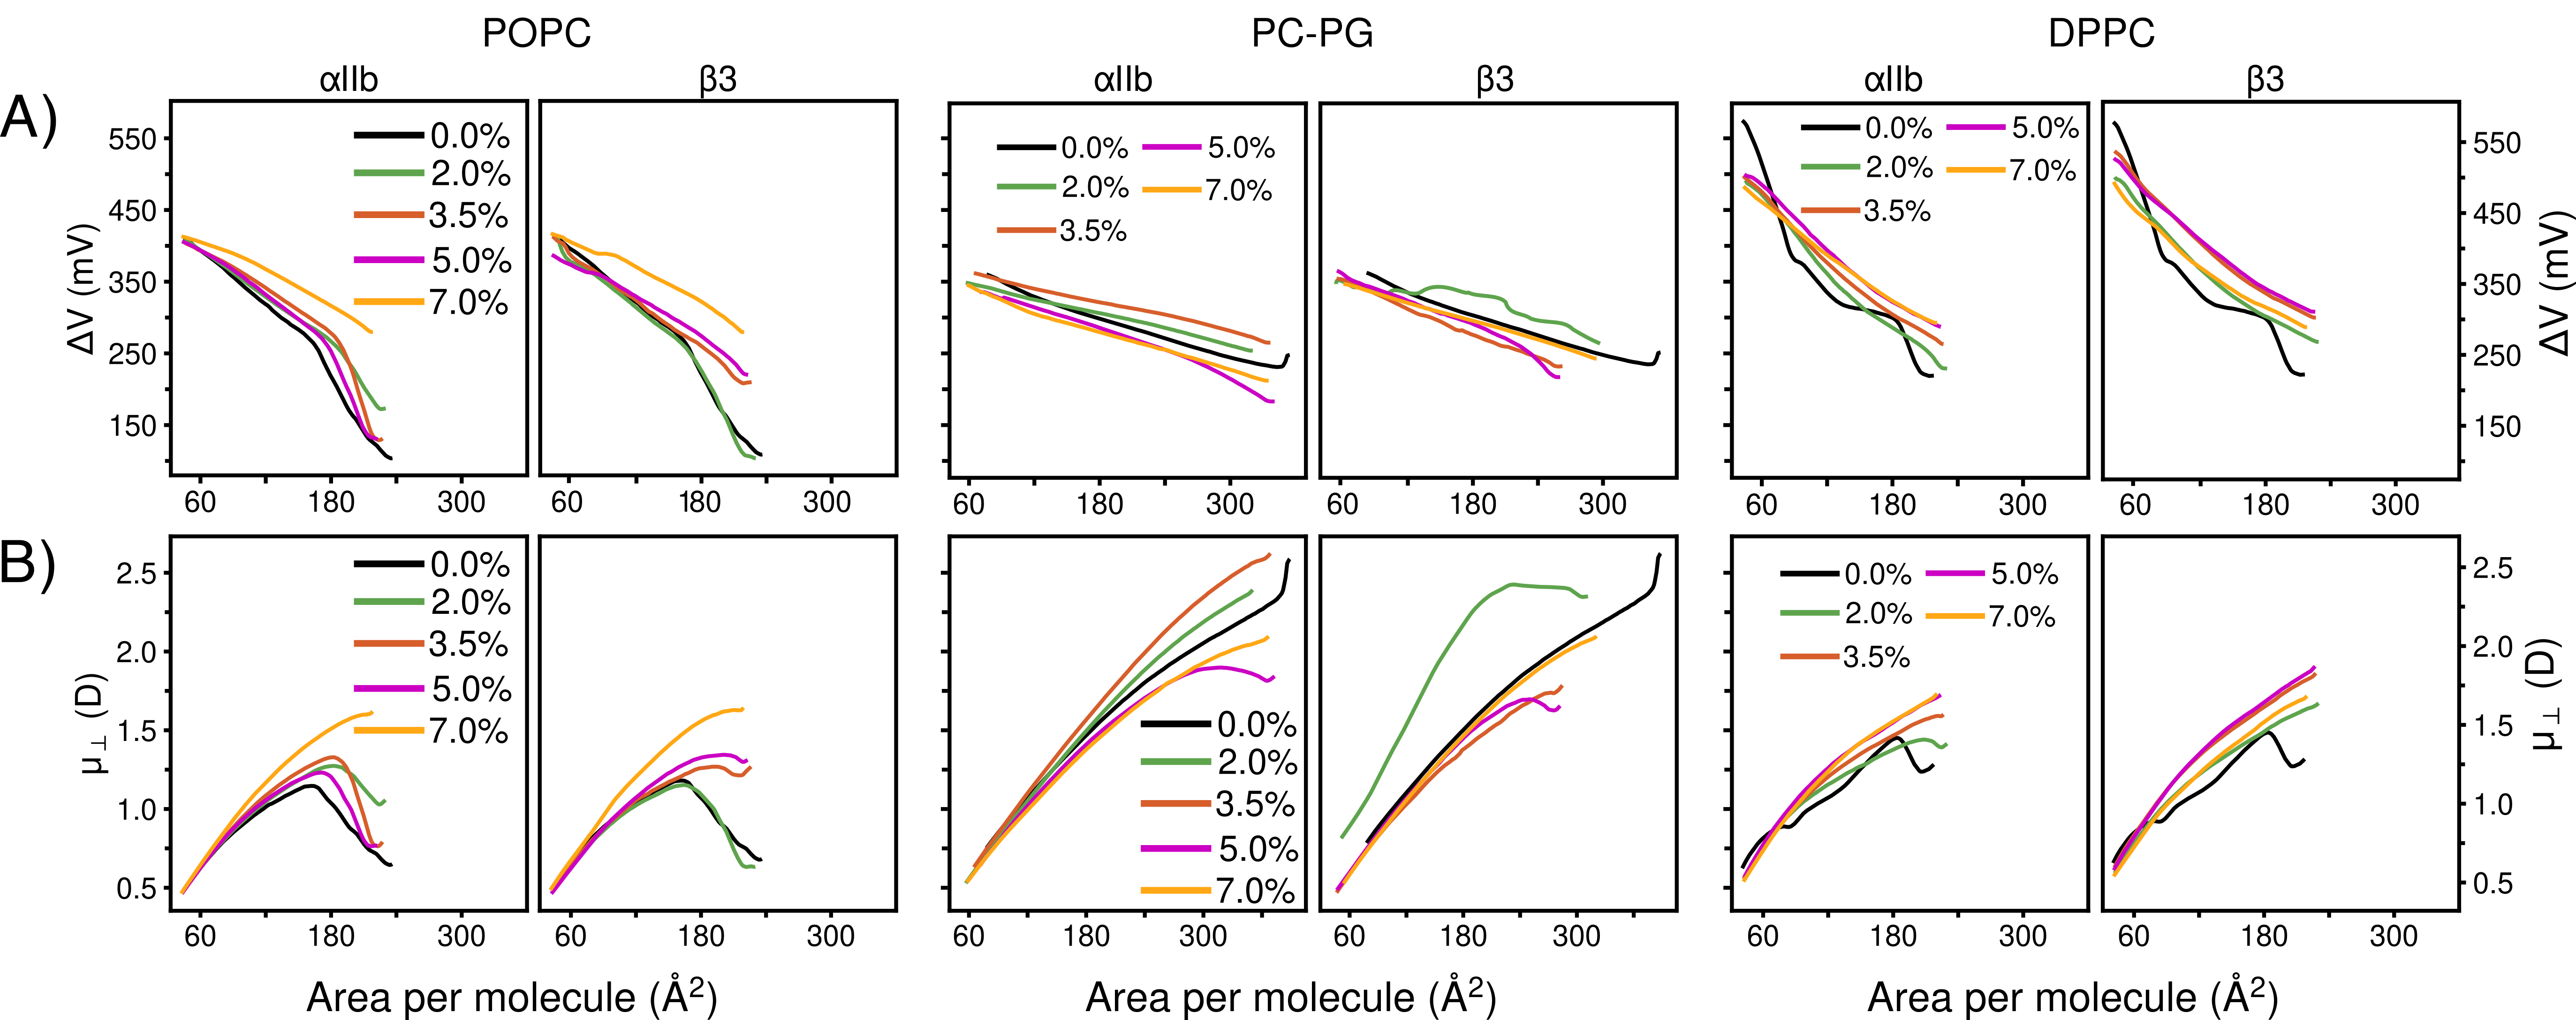
\includegraphics[width=0.99\linewidth, height=\textheight, keepaspectratio]{fig8.png}
\caption{A) Electric surface potential ($\Delta$\textit{V})  and B) apparent dipole moment ($\mu_\perp$) as a function of mean molecular area. Peptide mole fractions are represented by lines with different line colors.}
\label{fig:mu_dV_alfa}
\end{figure}
%%%%%%%%%%%% End %%%%%%%%%%%%

\noindent \textit{Mechanical Properties.}
The monolayer compressibility gives us information about the structure and molecular organization. Fluctuating molecules with large degrees of freedom should produce more compressible monolayers. The compressibility modulus \textit{C}$_s^{-1}$ is proportional to the derivative of the $\pi$–area isotherm according to: $C_s^{\text{–}1} =  \text{–} A \left(\frac{d\pi}{dA} \right) $. The larger \textit{C}$_s^{-1}$, the less compressible is the monolayer. Typical values for \textit{C}$_s^{-1}$ are 12–50 mN$\cdot$m$^{-1}$ for monolayers in the LE phase and 100–250 mN$\cdot$m$^{-1}$ for LC \cite{Davies1961}. \autoref{fig:Cs1} shows the \textit{C}$_s^{-1}$ values for pure lipids, pure peptides and the studied mixtures. Up to about 10 mN$\cdot$m$^{-1}$ of surface pressure, for both peptides, \textit{C}$_s^{-1}$ was small, corresponding to a compressible monolayer (further discussed below). Above 10 mN$\cdot$m$^{-1}$ of surface pressure \textit{C}$_s^{-1}$ increased to reach an average value of 35 mN$\cdot$m$^{-1}$ for peptide $\alpha$IIb and 25 mN$\cdot$m$^{-1}$ for peptide $\beta$3.

%%%%%%%%%%%% Figure %%%%%%%%%%%%
\begin{figure}[ht]
\centering
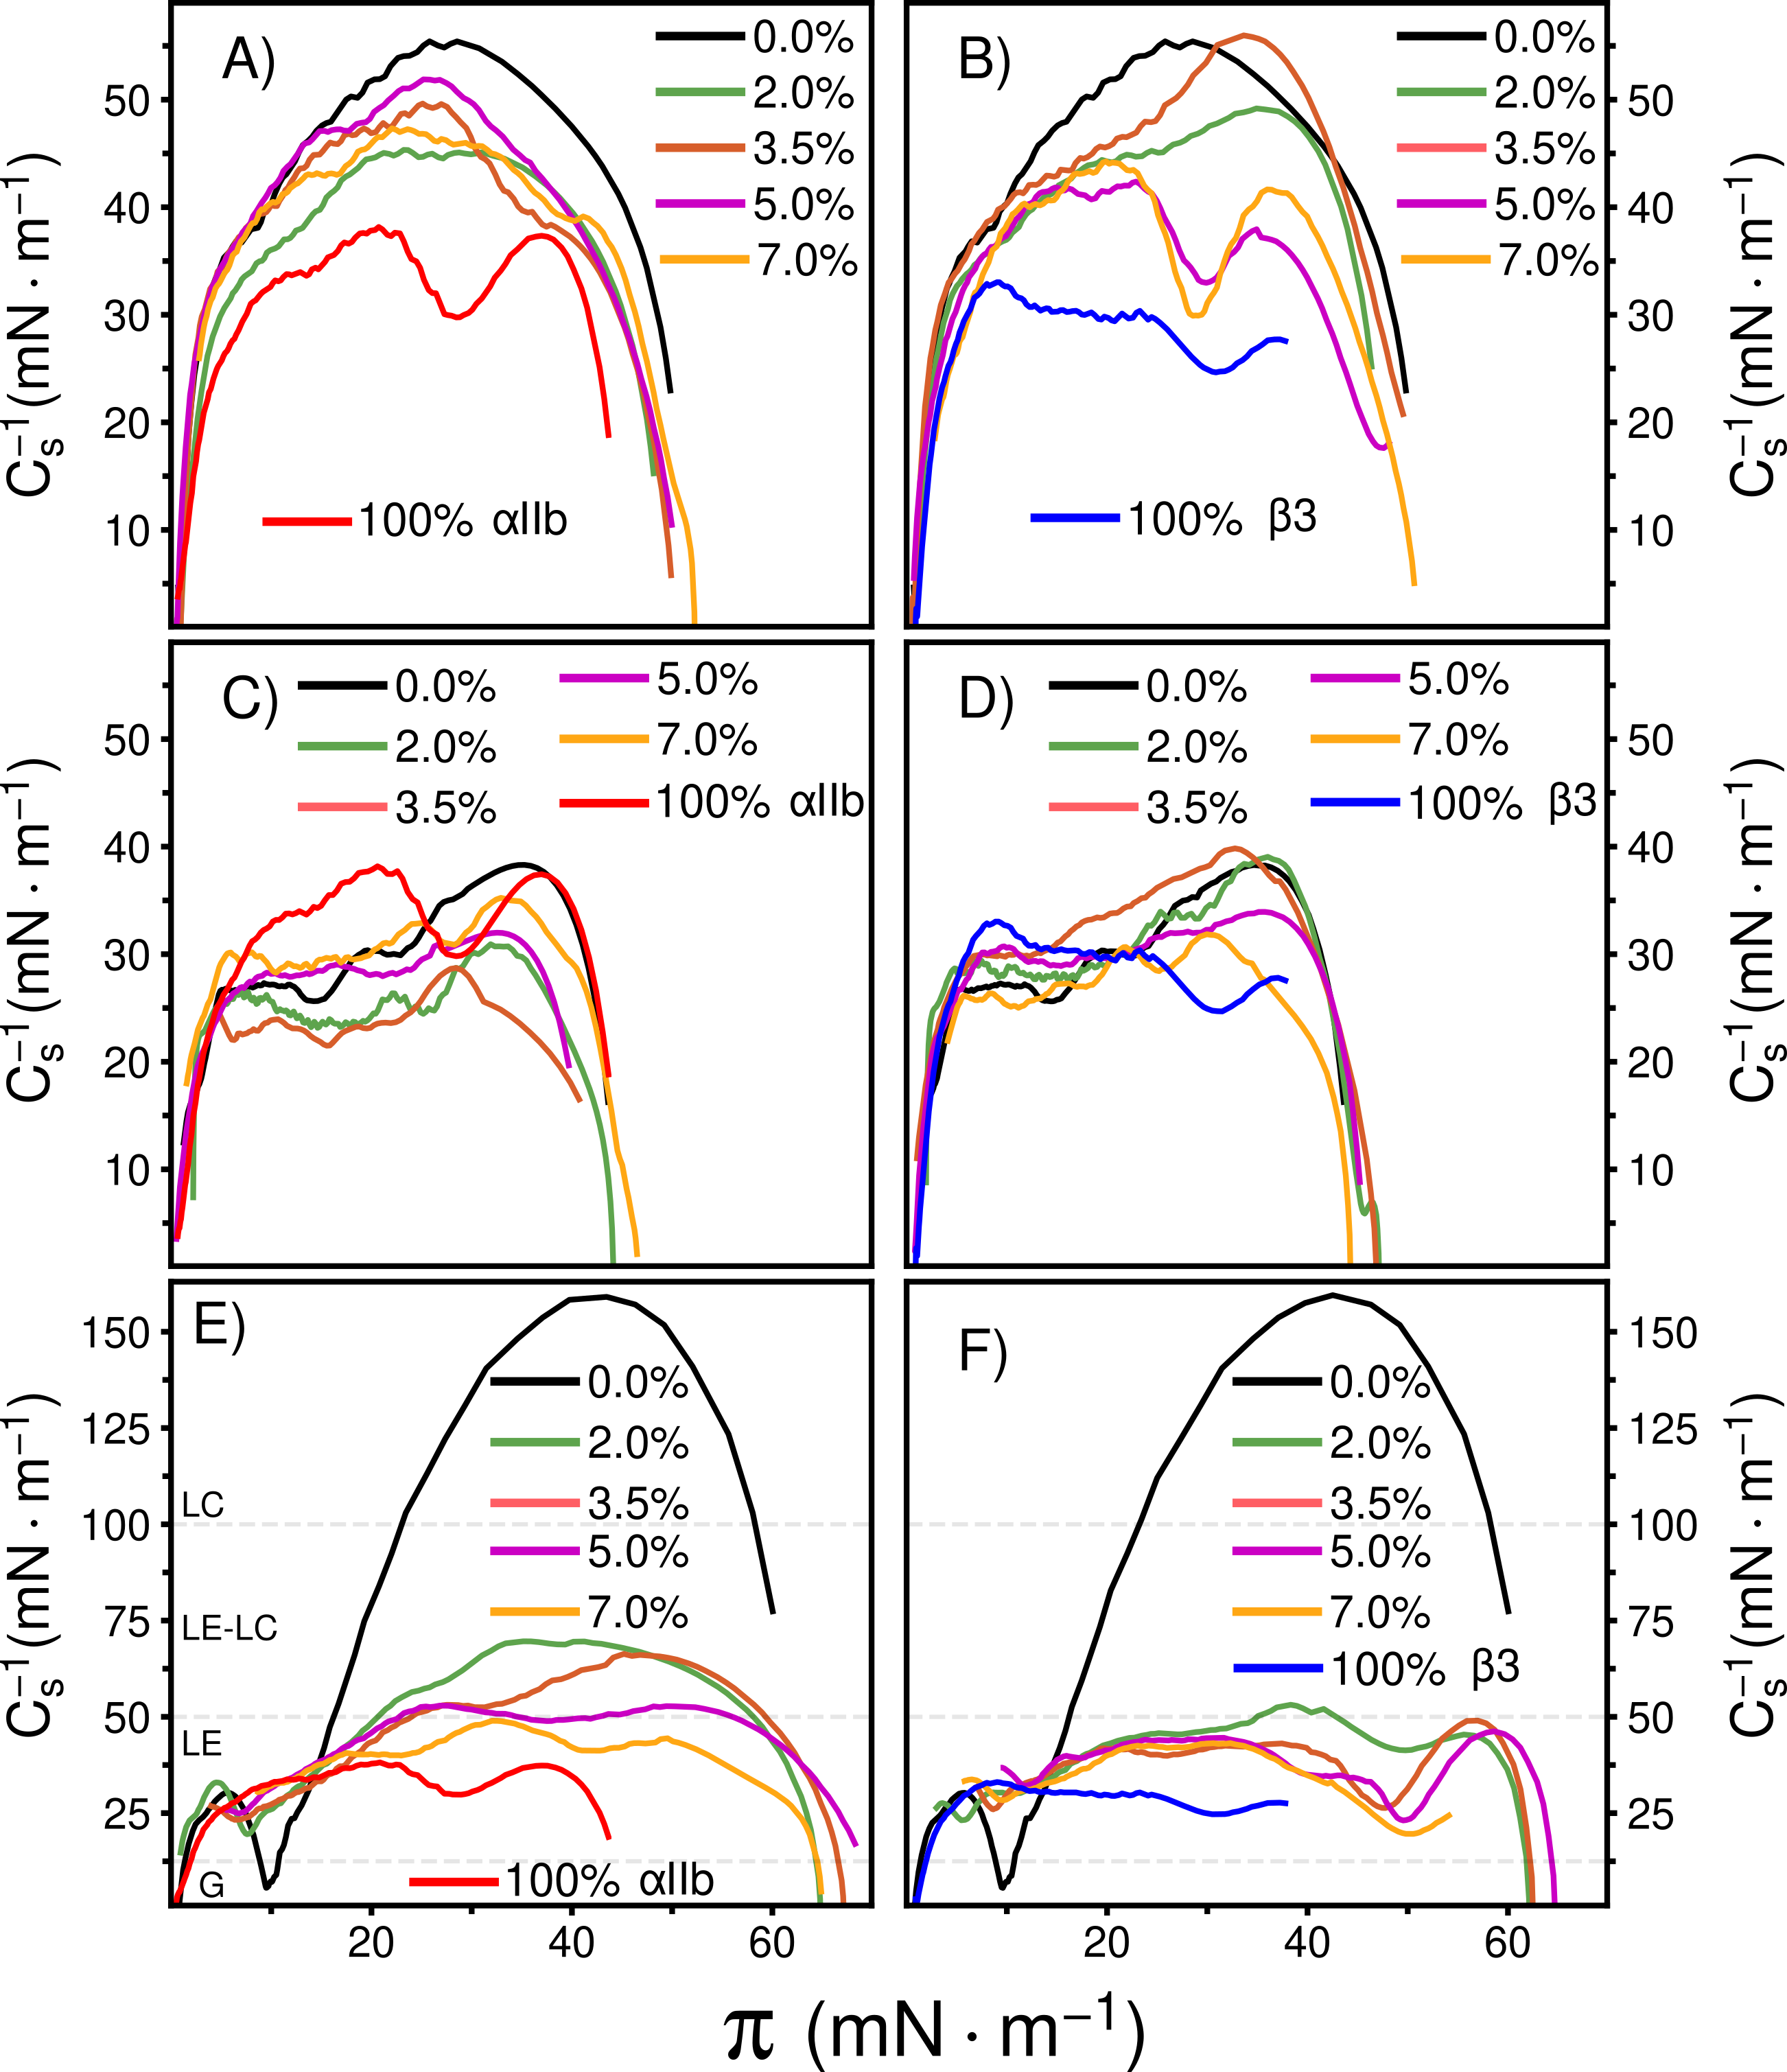
\includegraphics[width=0.6\linewidth, height=\textheight, keepaspectratio]{fig9.png}
\caption{Surface compressibility modulus as a function of surface pressure (\textit{C}$_s^{-1}$–$\pi$) for monolayers of pure lipids and their mixtures with different percentage of peptides.  A-B) POPC, C-D) PC–PG, E-F) DPPC. Peptide mole fractions ($\alpha$IIb  first column,  $\beta$3 second column) are represented by lines with different markers.}
\label{fig:Cs1}
\end{figure}
%%%%%%%%%%%% End %%%%%%%%%%%%

Pure peptides $\alpha$IIb and $\beta$3 showed a noticeable minimum in \textit{C}$_s^{-1}$ at 30 and 32 mN$\cdot$m$^{-1}$ surface pressure, respectively. Although this cannot be considered a first order phase transition, because \textit{C}$_s^{-1}$ did not approach to zero, it is a clear indication of a rearrangement of the monolayer. The compressibility of POPC decreased between $\pi$ = 0 and $\pi$ = 5 mN$\cdot$m$^{-1}$ (increasing values of \textit{C}$_s^{-1}$ from 0 to 30 mN$\cdot$m$^{-1}$) and further decreased with lower slope to reach \textit{C}$_s^{-1}$ = 50 mN$\cdot$m$^{-1}$. The mixture POPC–POPG instead, remained at about \textit{C}$_s^{-1}$ = 30 mN$\cdot$m$^{-1}$ after the first steep decrease in compressibility. DPPC, a compact monolayer of saturated lipid, reached high values of \textit{C}$_s^{-1}$ = 150 mN$\cdot$m$^{-1}$. The sharp minimum in the value of \textit{C}$_s^{-1}$ at $\pi$ = 10 mN$\cdot$m$^{-1}$ indicates a molecular reorganization of the monolayer including a phase transition.

Peptide $\alpha$IIb produced a small increase in the compressibility of POPC monolayer without changes in the shape of the curve. In the mixture with peptide $\beta$3 instead, also occurred a minimum \textit{C}$_s^{-1}$ at 30 mN$\cdot$m$^{-1}$ surface pressure, suggesting that the peptide, instead of the lipid, defined the compressibility of the monolayer. The shape of the curve and the compressibility values in the mixture PC–PG suffered little changes in the presence of the peptides. In DPPC, a large decrease in moduli was induced already at the lowest proportion of peptides. The mixtures of DPPC with lipids had \textit{C}$_s^{-1}$ corresponding to LE monolayers, in the whole range of the curve, suggesting the abolition of the LE–LC phase transition.\\


\noindent \textit{Morphology of the Films as Measured by BAM}.
In the previous sections we described and analysed the Langmuir monolayers of peptides and their mixtures with lipids following the classical treatment of compression isotherms, their variation of surface potential and compressibility and the deviation of the ideal mixing. These are macroscopic, average properties of the systems, that give us some clues about the organization of the interface and the interactions established between the components. Nevertheless, when drawing conclusions, we cannot a \textit{piori} suppose a homogeneous mixing, whether ideal or not, of the components. This is, we cannot suppose a model in which a peptide molecule is surrounded by lipids and draw conclusions about the detailed arrangement of these complexes. Actually, the following results with BAM shows that the peptide monolayers were heterogeneous in their arrangement and morphology.

Pure DPPC showed a homogeneous surface without observable structures in the liquid-expanded phase. Upon compression, the emerging liquid–condensed phase exhibited characteristic domains \cite{1997_Mcconlogue} (see \hyperref[sec:support]{Supplementary Figure S3}A), which begin to merge as the surface pressure increased, eventually leading to complete coalescence and the formation of a continuous LC phase with a homogeneous appearance. Pure POPC produced BAM images corresponding to a liquid–expanded isotherm at all surface pressures \cite{2020_Alvarez, 2022_Alvarez} (\hyperref[sec:support]{Supplementary Figure S3}B).

%%%%%%%%%%%% Figure %%%%%%%%%%%%
\begin{figure}[hb!]
\centering
\includegraphics[width=0.6\linewidth, height=\textheight, keepaspectratio]{fig10.png}
\caption{Representative BAM images of peptides $\alpha$IIb, $\beta$3 and their mixtures with POPC and DPPC. The monolayers were compressed at the indicated surface pressures. Pure peptide monolayers contained 0.75 nmol of $\alpha$IIb or $\beta$3. Mixed monolayers contained 20 nmol lipids + 0.005\% mole $\alpha$IIb or $\beta$3. Temperature was 20 $\pm$ 1 \textdegree C. All images have the same scale: 200 \textit{x} 252 $\mu$m$^2$. BAM images of pure lipids are shown in \hyperref[sec:support]{Supplementary Figure S3}. The contrast in the images has been adjusted to enhance visualization. In the lower right corner, the white bar represents the scale of 20 $\mu$m.}
\label{fig:bam}
\end{figure}
%%%%%%%%%%%% Fin %%%%%%%%%%%%

\autoref{fig:bam} shows the BAM images of pure peptides and their mixtures with POPC and DPPC. Lipid–peptides mixtures contained 0.005 mol\% of peptide. Under the present BAM experimental conditions, larger proportions of peptides produced a large increase in surface pressure and a large coverage of saturationg, brilliant domains. At very low surface pressure, 2 mN$\cdot$m$^{-1}$, both peptides displayed a homogeneous field (not shown). At 5 mN$\cdot$m$^{-1}$ they organized in the interface as threads of large reflectivity. These threads were largely connected in a continuous net with some short ramifications. As the surface pressure increased to 15 mN$\cdot$m$^{-1}$ the threads were laterally concentrated, occupying a larger relative area and maintaining their general shape. A difference was observed between $\alpha$IIb and $\beta$3 at 15 and 20 mN$\cdot$m$^{-1}$: while $\alpha$IIb followed the same trend with the increase in surface pressure, the threads of $\beta$3 showed a larger increase in reflectivity and large patches of continuous high reflectivity, that is, patches instead of threads. Besides, at 15 and 20 mN$\cdot$m$^{-1}$ of the $\beta$3 peptide, the dark areas were populated with round domains of intermediate reflectivity (\autoref{fig:bam}). For both peptides, at low surface pressure, 5 mN$\cdot$m$^{-1}$, it can be observed that the dark phase was not homogeneous. Dark round patches of reflectivity values close to the pure water were surrounded by a percolating phase of slightly larger reflectivity. A detailed observation shows that the bright threads start exclusively in the continuous, less reflective phase (see zoom in \autoref{fig:bam}).

A remarkable change in the peptide domains was observed in the mixtures with DPPC. Already at 5 mN$\cdot$m$^{-1}$ instead of continuous threads as observed for pure peptides, they were shorts, discontinuous and unconnected. The increase of surface pressure produced an enrichment of these short, elongated domains without a major “reconnection”. The same effect was observed for both $\alpha$IIb and $\beta$3 peptides. In the mixtures with POPC the peptide domains were also different as compared with the pure peptides but the effect was smaller than observed in the mixtures with DPPC. In POPC the threads were continuous as in the pure peptides but more separated and covering lower areas than the pure peptides as the surface pressure increased.

\autoref{fig:thickness} shows the thickness of the peptide domains in the \textit{z} direction at different surface pressures for pure peptides and their mixtures with POPC and DPPC films, respectively. The values for the peptides were obtained by sampling three arbitrary regions for each frame as described in \hyperref[sec:support]{Supplementary Section S3 and Figure S4}. At 20 mN$\cdot$m$^{-1}$ we already observed some saturated values of reflectivity. Consequently, we only evaluated the thickness up to 15 mN$\cdot$m$^{-1}$. The thickness obtained for the pure peptides, $\sim$15 to $\sim$35 Å at 5 and 20 mN$\cdot$m$^{-1}$ respectively, were below the values expected for the peptides oriented perpendicular to the interface \cite{2005_Castano, 2015_Kato} (\autoref{fig:thickness}A). The extrapolation of these three points suggests that at 24 mN$\cdot$m$^{-1}$ for $\alpha$IIb and at about 30 mN$\cdot$m$^{-1}$ for $\beta$3 the bright domains can reach the thickness of 70 and 90 Å expected for vertically oriented peptides. The fact that the thickness of the bright domains changed with the surface pressure indicates that they are dynamic structures, able to reorganize whether by recruitment of material or tilting of ordered molecules. In any case, we cannot ascertain if, microscopically, the domains are an amorphous or a crystalline collection of peptides. In the mixtures with lipids, the peptide domains did not show large changes in their thickness, only POPC produced a significant decrease in the thickness of $\alpha$IIb and only at surface pressures of 5 and 10 mN$\cdot$m$^{-1}$ (\autoref{fig:thickness}A).

Above 20 mN$\cdot$m$^{-1}$ the images of BAM did not provide reliable information because of a large, saturated and almost homogeneous reflectivity. We were not able to identify domains of different reflectivity above 20 mN$\cdot$m$^{-1}$. For this reason, it was not possible to use BAM data to correlate directly with the rearrangement at about 30 mN$\cdot$m$^{-1}$ revealed by the compressibility in \autoref{fig:Cs1} (see \hyperref[sec:discu]{Discussion} below).

%%%%%%%%%%%% Figure %%%%%%%%%%%%
\begin{figure}[h!]
\centering
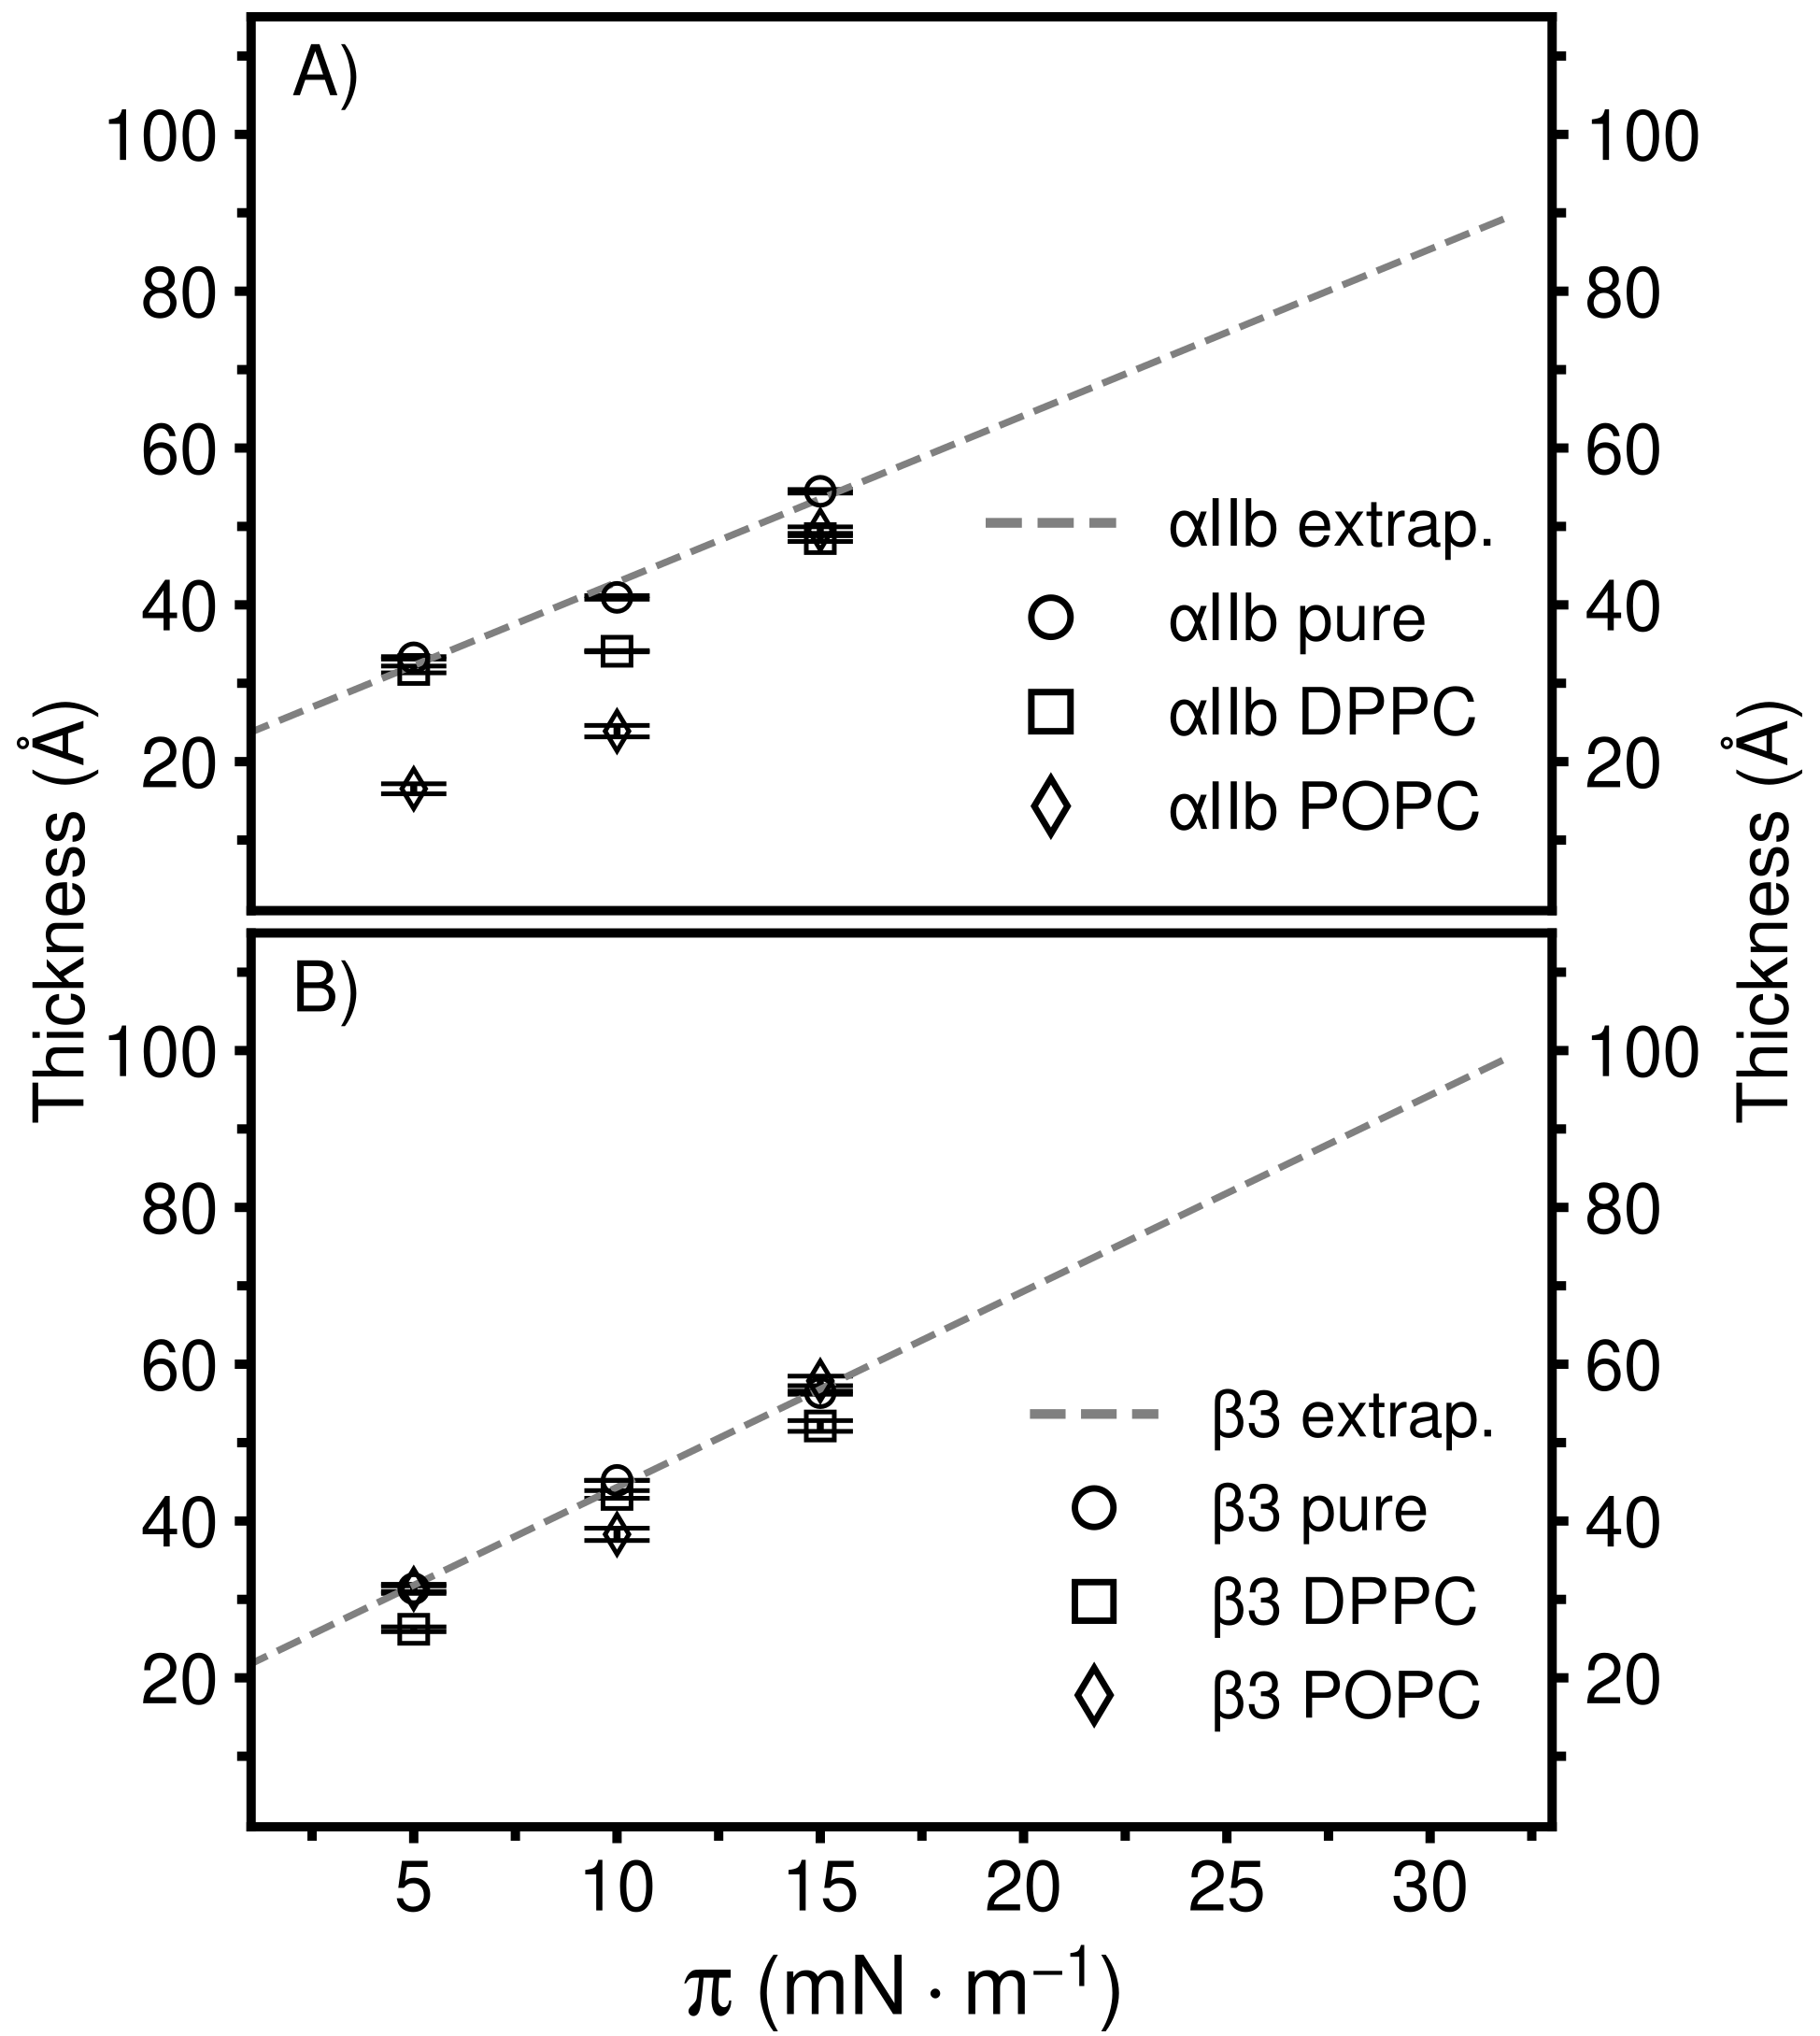
\includegraphics[width=0.5\linewidth, height=\textheight, keepaspectratio]{fig11.png}
\caption{Monolayer thickness from BAM images of pure peptides and their mixtures with lipids. Panel A: $\alpha$IIb. Panel: B $\beta$3. Circles: pure peptides; squares: mixtures with DPPC; diamonds: mixtures with POPC.}
\label{fig:thickness}
\end{figure}
%%%%%%%%%%%% Fin %%%%%%%%%%%%

The difference in the lateral organization of peptides in DPPC as compared with POPC, revealed by the difference in the thickness of the clear phases, was in agreement with the fact that the mixtures with these lipids showed different mixing behaviour as described in \autoref{fig:mixIsothe} and \autoref{fig:areaIdealMix} and in the Supplementary \hyperref[sec:support]{Supplementary Figure S5C,F}.

%%%%%%%%%%%%%%%%%%%%%%%%%%%%%%%%%%%%%%%%%%%%%%%%%%%%%%%%%%%%%%%%%%%%%
\section{Discussion}\label{sec:discu}

A major point in the discussion of our results is to what extent they can be related to the integrin TM domains-lipid interactions in the actual plasma membrane. The correlation between monolayers and bilayers has been largely discussed from the general thermodynamic and structural point of view and also for several particular systems including peptides and proteins (see for example the reviews by Rosetti et al. \cite{2008_Rosetti} and by Möhwald \cite{1990_Mohwald}). In general, the lack of rigorous similarity is compensated by the capability of monolayers to control the compactness and geometry of the system and to precisely measure the dipolar organization, compressibility and thickness. We did not expect a \textit{priori} to reproduce in monolayers the interactions and the organization of the TM segments occurring in the bilayer. Actually, in the monolayers, the peptides were self–organized in domains that are not representative of the organization of the whole protein in the cell membrane. Then, what we can obtain from these monolayers studies are basic principles regarding the influence of the peptides on the lipid organization and the capability of different lipids to interact with the TM segments.

The classical interpretation of surface pressure as a function of the area isotherms suggest that, if the peptides were forming homogeneous monolayers they would be acquiring a mixture of orientations, including horizontal in the plane of the membrane, tilted and probably a fraction of vertical orientations. The visualization of complex domains obtained in the BAM experiments indicated a much more complex scenario in terms of possible orientations and interactions with lipids. This precludes us from interpreting the results on the basis of a model of $\alpha$–helix cylinders surrounded by lipids as expected for the organization in the plasma membrane. The information that we can obtain from the present experiments clearly do not describe directly how the peptides interact with lipids in the real plasma membrane. Instead, we can evaluate what can be considered intrinsic capability of peptides–lipids interactions.

We have found several valuable data about the interactions of the TM segments of integrin $\alpha$IIb$\beta$3 with lipids. In the first place we find that both peptides tend to interact between themselves better than with lipids, this is concluded because the organization of pure peptides as threads in the interface is basically preserved in the mixed monolayers according to the BAM images. In this regard, the saturated lipid DPPC seems to establish more favourable interactions with the TM peptides because it can disassemble, to some extent, peptide–peptide interactions producing interrupted threads of high reflectivity. Besides, the influence of the peptides on the behaviour of the lipid, even at low proportions, was remarkable: DPPC behaved as a fluid lipid and did not go through a phase transition in the presence of the peptides. It is interesting to consider that the positive deviation of ideal mixing with DPPC was because this lipid was not able to reach the condensed state in the presence of the peptides, giving as a consequence a larger area. The unsaturated POPC was less effective in disrupting the peptides threads. Even when the proportion of peptide was much lower for the BAM experiments, this observation is in line with the proposal that in the mixtures with POPC the peptide define the elastic properties of the monolayer, at least for the case of $\beta$3. This is a clear indication that, in general, different lipids can have differential interactions with TM segments producing differential organization in the lipid bilayer and have influence on the functionality of the integrin.

To explain the variations of compressibility with the surface pressure we should take into account that the peptides were organized in separate domains, particularly in the shape of a network. When two phases are present, the surface compressibility of the monolayer is a linear combination of the compressibility of the existing phases. To quantify these contributions, a phase diagram is required \cite{2013_Caruso}. We cannot directly relate the compressibility data (\autoref{fig:Cs1}) with the BAM images because we were not able to produce images at the relatively large proportion of peptide used in the compressibility measurements. Nevertheless, we can find an interesting correlation: only in the $\beta$3 peptide–POPC mixtures the compressibility can follow the profile of the pure peptide with the reorganization observed at 30 mN$\cdot$m$^{-1}$ (\autoref{fig:Cs1}B, 5 and 7\% peptide) coincidently with the observation that the brilliant threads are more continuous than in the other mixtures ($\alpha$IIb–POPC, and the largely discontinuous $\alpha$IIb–DPPC, $\beta$3–DPPC, \autoref{fig:bam}). It could be proposed that the connectivity is required to transmit the compressibility of the phase to the whole system. If this were the case we could speculate that it is not the intrinsic compressibility of the phase but rather the compressibility of the network that define the mechanical property of the system.
The percolation threshold is the condition, as a function of composition, surface pressure or other variables, at which all sites of the lattice in one phase are connected. In this regard, the brilliant phases in pure peptides and in the mixtures with POPC, particularly in the $\beta$3–POPC mixture, were above the percolation threshold.  Risović  et al.\cite{2011_Risovic} have shown that at the percolation threshold occurs a sharp increase in the compressibility modulus. We were not able to study this behaviour of the compressibility because the brilliant phases of pure peptides and their mixtures with POPC, when visible, were already above the percolation threshold.

\section{Conclusions}
We expressed and purified segments of the integrin $\alpha$IIb$\beta$3 protein and studied the surface behavior of the pure peptides and their mixtures with lipids in Langmuir monolayers. Both peptides presented a significant interfacial activity at the air/water interface, forming stable monolayers. The amphiphaticity profile of the peptides suggested that the IC segments were located in the aqueous environment. From the calculated $\lambda$–factor used to study lateral miscibility in mixtures, we concluded that the differences between the experimental and ideal isotherms of POPC and PC–PG are solely attributed to the value of $\lambda$ and are independent of the surface pressure (with r$^2$ > 0.85). This indicates that interactions between peptides and the lipids in the LE phase are similar along the compression isotherm. In the mixtures with DPPC this analysis was in agreement with the large difference between the shape of pure DPPC and mixed monolayer.

Pure peptide monolayers reorganized as a function of the surface pressure as showed by the changes in compressibility. The presence of either $\alpha$IIb or $\beta$3 peptides increased the compressibility of lipid monolayers and eliminated the phase transition of DPPC.

Pure peptides produced BAM images that followed a pattern of continuous, connected threads or strings of high reflectivity with ramifications. These patterns of high reflectivity grew from a continuous, percolating phase of low reflectivity surrounding round dark patches. In the mixtures with DPPC, the peptide threads were discontinuous. According to the compression isotherms, these mixtures with DPPC occupy an area larger than the expected for the ideal mixing. The interactions with POPC were remarkable different because the threads were much less interrupted and the deviations from the ideal mixing were negative. The data presented in this paper show that the surface, mechanical, and topographical characteristics of lipid films can be regulated by the $\alpha$IIb or $\beta$3 TM segments of the integrin and that these segments can establish differential interactions with lipids.

%%%%%%%%%%%%%%%%%%%%%%%%%%%%%%%%%%%%%%%%%%%%%%%%%%%%%%%%%%%%%%%%%%%%%

\subsection*{Associated Content}\label{sec:support}
\textbf{Supporting Information}

\noindent Section S1: Protein expression and purification methods\\
Figure S1: Protein characterization \\
Figure S2: The amino acid sequences and structures of integrin individual $\alpha$IIb and $\beta$3 TM–IC segments\\
Section S2: Infrared bands identification and fitting\\
Table S1: Components of the amide I band of $\alpha$IIb and $\beta$3 peptides \\
Section S3: Quantitative analysis of BAM images\\
Figure S3: BAM images of DPPC and POPC pure monolayer subphases\\
Figure S4: Sampling the region of interest (ROI) to determine the thickness of the brilliant threads\\
Figure S5: Mean molecular area as a function of the molar fraction of the peptide at 15 and 20 mN$\cdot$m$^{-1}$


\subsection*{Author Information}\label{sec:authors}
\subsubsection{Corresponding Author}
*E-mail: guillermo.montich@unc.edu.ar, Phone/Fax: +54 351 4334171

\begin{acknowledgement}
This work was supported by grants from SECyT–UNC (Res. SeCyT 91/19), FONCyT (PICT–2015–1612) and Departamento Administrativo de Ciencia, Tecnología e Innovación (Colciencias, Grant 860–2019), Colombia. U.C.S. was a fellow of CONICET and FONCyT. A.G., J.L.B., G.R.O. and G.G.M. are career members of CONICET. The authors thank to Jun Qin and Jun Yang for kindly providing the peptide plasmids, to “Sistema Nacional de Microscopía” and “Sistema Nacional de Grandes Instrumentos”, Argentina. We also thank to Carla Rossetti, Luis B. Socas, Natalia Wilke, Martín Villanueva and Maria Elena Carrizo for helpful discussion. Ing. Marcelo Pino is in charge of technical support and maintenance of BAM facility.
\end{acknowledgement}

\bibliography{referen}
\end{document}